% mnras_template.tex
%
% LaTeX template for creating an MNRAS paper
%
% v3.0 released 14 May 2015
% (version numbers match those of mnras.cls)
%
% Copyright (C) Royal Astronomical Society 2015
% Authors:
% Keith T. Smith (Royal Astronomical Society)

% Change log
%
% v3.0 May 2015
%    Renamed to match the new package name
%    Version number matches mnras.cls
%    A few minor tweaks to wording
% v1.0 September 2013
%    Beta testing only - never publicly released
%    First version: a simple (ish) template for creating an MNRAS paper

%%%%%%%%%%%%%%%%%%%%%%%%%%%%%%%%%%%%%%%%%%%%%%%%%%
% Basic setup. Most papers should leave these options alone.
\documentclass[a4paper,fleqn,usenatbib]{mnras}

% MNRAS is set in Times font. If you don't have this installed (most LaTeX
% installations will be fine) or prefer the old Computer Modern fonts, comment
% out the following line
\usepackage{newtxtext,newtxmath}
% Depending on your LaTeX fonts installation, you might get better results with one of these:
%\usepackage{mathptmx}
%\usepackage{txfonts}

% Use vector fonts, so it zooms properly in on-screen viewing software
% Don't change these lines unless you know what you are doing
\usepackage[T1]{fontenc}
\usepackage{ae,aecompl}


%%%%% AUTHORS - PLACE YOUR OWN PACKAGES HERE %%%%%

% Only include extra packages if you really need them. Common packages are:
\usepackage{graphicx}	% Including figure files
\usepackage{amsmath}	% Advanced maths commands
\usepackage{amssymb}	% Extra maths symbols
\usepackage[]{algorithm2e}
\usepackage[caption=false]{subfig}
\graphicspath{{figures/}}

%%%%%%%%%%%%%%%%%%%%%%%%%%%%%%%%%%%%%%%%%%%%%%%%%%

%%%%% AUTHORS - PLACE YOUR OWN COMMANDS HERE %%%%%

% Please keep new commands to a minimum, and use \newcommand not \def to avoid
% overwriting existing commands. Example:
%\newcommand{\pcm}{\,cm$^{-2}$}	% per cm-squared

%%%%%%%%%%%%%%%%%%%%%%%%%%%%%%%%%%%%%%%%%%%%%%%%%%

%%%%%%%%%%%%%%%%%%% TITLE PAGE %%%%%%%%%%%%%%%%%%%

% Title of the paper, and the short title which is used in the headers.
% Keep the title short and informative.
\title[Hierarchical Triples]{Waveforms from Hierarchical Triples for LISA}

% The list of authors, and the short list which is used in the headers.
% If you need two or more lines of authors, add an extra line using \newauthor
\author[T. Kimpson et al.]{
 Kimpson,$^{1}$\thanks{E-mail: tom.kimpson.16@ucl.ac.uk}
Huan Yang  ,$^{2}$
\\
% List of institutions
$^{1}$ Mullard Space Science Laboratory, University College London. Holmbury St. Mary, Dorking, Surrey, RH5 6NT, UK, \\
$^{2}$ PI, Canada, etc
}


% These dates will be filled out by the publisher
\date{Accepted XXX. Received YYY; in original form ZZZ}

% Enter the current year, for the copyright statements etc.
\pubyear{2019}

% Don't change these lines
\begin{document}
\label{firstpage}
\pagerange{\pageref{firstpage}--\pageref{lastpage}}
\maketitle

% Abstract of the paper
\begin{abstract}
blah blah blah
\end{abstract}

% Select between one and six entries from the list of approved keywords.
% Don't make up new ones.
\begin{keywords}
gravitation -- pulsars -- black hole physics
\end{keywords}

%%%%%%%%%%%%%%%%%%%%%%%%%%%%%%%%%%%%%%%%%%%%%%%%%%

%%%%%%%%%%%%%%%%% BODY OF PAPER %%%%%%%%%%%%%%%%%%

\section{Introduction}
Intro...

\noindent What are the waveforms from $\sim$ stellar mass BH binaries in hierarchical triple systems, as detected by LISA. Especially those which retain significant eccentricities.

\section{Waveform model}
We now discuss how to construct a waveform model for gravitational waves from BH binaries in the LISA band...



\subsection{Equations of motion}

In specifying the equation of motion of the inner binary we adopt the formalism of \citep{Randall2018}. Within this framework the evolution of the orbital elements has contributions from the Kozai-Lidov mechanism in addition to the usual PN precession of periastron and relativistic corrections due to the emission of gravitational radiation. In order to properly model the waveforms from astrophysical HT systems across a general parameter space, it is important to consider the convolution of both the KL and GW radiative effects. Whilst for specific configurations the KL effects can dominate over the GW ones, more generally the GW effects act to dampen the impact of KL oscillations. To construct a general, accurate model to explore the impact of KL oscillations on the resultant waveform requires a consistent approach to modelling both these effects. \newline 

\noindent The KL, GW and PN effects imprint on the evolution of 4 key variables of the inner binary: the eccentricity $e$, the semi-major axis $a$, the pericentre angle $\gamma$ and the orbital angular momentum $J$. The complete set of coupled ODEs for the evolution of the orbital parameters are \citep{Randall2018},
\begin{eqnarray}
\dot{e} = \dot{e}_{\rm KL} + \dot{e}_{\rm GW}
\label{eq:edot}
\end{eqnarray}
\begin{eqnarray}
\dot{\gamma} = \dot{\gamma}_{\rm KL} + \dot{\gamma}_{\rm PN}
\end{eqnarray}
\begin{eqnarray}
\dot{a} = \dot{a}_{\rm GW} 
\label{eq:gwdot}
\end{eqnarray}
\begin{eqnarray}
\dot{J} = \dot{J}_{\rm GW} 
\label{eq:gwdot}
\end{eqnarray}
where the eccentricity components are
\begin{eqnarray}
\dot{e}_{\rm KL} =   \frac{\mathcal{A} a^2 e u(e)}{J}  \sin 2 \gamma
\end{eqnarray}
\begin{eqnarray}
\dot{e}_{\rm GW} = \frac{19}{12} \mathcal{C} a^{-4} g(e)
\end{eqnarray}
the $\gamma$-components:
\begin{align}
\dot{\gamma}_{\rm KL} = 2 Ka^2\left[\frac{1}{J_{1}}\left(2u(e)-5 \sin ^{2} \gamma_{1}\left(u(e)-\cos ^{2} I\right) \right)\right. \\
\left.+\frac{\cos I}{J_{2}}\left(u(e)+5 e_{1}^{2} \sin ^{2} \gamma_{1}\right) \right]
\end{align}
\begin{eqnarray}
\dot{\gamma}_{\rm PN} = \lambda a^{-2.5} u^{-1 }
\end{eqnarray}
the evolution of $a$:
\begin{eqnarray}
\dot{a}_{\rm GW} = \mathcal{C} a_{1}^{-3} f(e_1)
\end{eqnarray}
and of the angular momentum:
\begin{eqnarray}
\dot{J} = \eta a^{-7/2} (1-e^2)^{-2} h(e)
\end{eqnarray}
The constants are defined as:
\begin{align}
\mathcal{C} &= -64 G^{3} \mu m^{2} / 5c^5 \\
\mathcal{A} &= 5 K \left(1-\cos ^{2} I\right) \\
\lambda &= 3/c^2 (Gm)^{3/2} \\
K &= \frac{3 G m_{0} m_{1} m_{2}}{8 M} \frac{1}{a_{2}^{3}\left(1-e_{2}^{2}\right)^{3 / 2}} \\
\eta &= -\frac{32}{5} \frac{G^{7/2} \mu m^{5/2}}{c^5}
\end{align}
whilst the eccentricity functions are given by
\begin{eqnarray}
g(e) = \frac{e}{\left(1-e^{2}\right)^{5 / 2}}\left(1+\frac{121}{304} e^{2} \right)
\end{eqnarray}
\begin{eqnarray}
f(e) = \frac{1}{\left(1-e^{2}\right)^{7 / 2}}\left(1+\frac{73}{24} e^{2}+\frac{37}{96} e^{4}\right)
\end{eqnarray} 
\begin{eqnarray}
h(e) = 1 + \frac{7}{8} e^2
\end{eqnarray} 
\begin{eqnarray}
u(e) = 1 - e^2
\end{eqnarray} 
We use the subscripts $2$ denote variables which relate to the outer binary, and $I$ is the inclination of the inner orbit relative to the outer orbit. \newline 



\noindent It is possible to solve this set of ODEs numerically to determine the evolution of the binary. However, given the length of the LISA mission ($T \sim 5$ years) and the broad parameter space we wish to explore, it quickly becomes computationally intractable to compute waveforms to sufficient precision in this way. Instead we seek an analytical or semi-analytical approach. Naturally such an method loses something in accuracy compared to the full numerical evolution, but we will show that our approximations which allow an analytical model to be constructed are appropriate and serve to capture the key physics of the systems we wish to investigate. In particular, the characteristic feature of hierarchical triples as distinct from other binaries is the presence of KL oscillations and it is the impact of these on the waveform, in conjunction with other relativistic effects that we wish to model and explore. \newline


\subsection{Constructing a model}





\subsubsection{A simple model}
\noindent To construct an analytical solution we make the following approximations:
\begin{enumerate}
	\item Linearity of pericentre evolution.$\gamma(t) = \dot{\gamma}_0 t + \gamma_0$.
	\item Linearity of semi major axis evolution $a(t) = \dot{a}_0 t + a_0$.
	\item Two-timescale decomposition of $e(t)$
\end{enumerate}
where $\dot{\gamma}_0 = \dot{\gamma} (t=0)$ , $\dot{a}_0 = \dot{a} (t=0)$\newline 



\textbf{CANONICAL}


\noindent Regarding the first two approximations, we are concerned here with (hierarchical) BH-BH binaries which fall in the LISA band. Such systems are different from e.g. LIGO BH-BH mergers or LISA EMRIs since they are far from merger and can retain medium eccentricities. As a consequence the second time derivatives of $\gamma(t), a(t)$ are typically small and their evolution is well approximated by a simple linear function. To further illustrate the point, in Figure \ref{fig:eg_exampleB10} we present the numerical evolution of orbital parameters. We consider a typical hierarchical triple system, of the sort that could be detectable with LISA, where $m_0 = m_1 = 30 M_{\odot}$, $m_2 = 10 M_{\odot}$, orbital frequency $f =10^{-3}$ Hz, $e_1 = 0.5$, $e_2 = 0.6$, and inclination $I = 60 \deg$. We quantify the separation of the inner and outer binary via the parameter $\beta = a_2/a_1$. In both the $\beta = 10$ and $\beta = 100$ cases, the evolution of $\gamma$ follows a clear linear relationship with time ($a(t)$ exhibits the same linear behaviour). This relation holds despite the marked difference in the behaviour of the eccentricity; in the $\beta=10$ case the eccentricity exhibits large amplitude sinusoidal variations. Conversely in the more separated case the amplitude of the eccentricity is markedly reduced and the combination of the oscillations induced by the KL mechanism with the secular decrease due to the GW emission circularising the binary are clearly visible. \newline 


\noindent We can now write,
\begin{eqnarray}
\frac{1}{e_1(1-e_1^2)}\dot{e} = \mathcal{A} a_1^2 \sin 2 \gamma_{1} + \frac{19}{12} \mathcal{C} a_1^{-4} h(e_1)
\label{eq:edotter}
\end{eqnarray}
where  we have defined  $h(e) = g(e) e^{-1} (1-e^2)^{-1}$.  This is not generally integrable since the $h(e_1)$ function spoils the separability of the expression. The equation becomes integrable if we neglect the time dependence of this function and approximate it as $h(e_1) \sim h(e_0)$. This approximation is effectively a recognition that the evolution of $e(t)$ occurs on two different timescales; a oscillatory short timescale due to the KL contributions (first term on RHS of Eq. \ref{eq:edotter}) and a linear longer timescale due to the GW contributions. This $h(e_1) \sim h(e_0)$ approximation is well justified for the sorts of systems considered in this work. $h(e)$ is maximal for high eccentricities (singular at $e=1$). For the system considered above $h(0.9) \sim 400$. The exponential nature of $h(e)$ means that for more moderate eccentricities $h(e)$ is much reduced, e.g. $ h(0.5) \sim \mathcal{O} (1)$. In contrast $|\mathcal{C}| \sim 10^{24}$ and so in evaluating the second term on the RHS, in comparison $h(e)$ can be taken as constant as the orbit evolves. In this case Eq. \ref{eq:edotter} can be solved exactly via separation of variables as, 
\begin{eqnarray}
e(t) = \frac{\exp (\alpha)}{\sqrt{1 + \exp (2 \alpha)}}
\end{eqnarray}
where 
\begin{eqnarray}
\alpha = \mathcal{A} \psi - \frac{19}{36} \frac{\mathcal{C} h(e_0)}{\dot{a}_0 a^3} + D
\end{eqnarray}
where,
\begin{align}
\psi = \frac{1}{4 \dot{\gamma}_0} \Bigg ( - 2a_0^2 \dot{\gamma_0^2} \cos2 \gamma + 2 a_0 \dot{a}_0 \dot{\gamma}_0 \left[-2t \dot{\gamma}_0 \cos 2 \gamma \right] \\
+ \dot{a}_0^2 \left[\cos 2 \gamma - 2t^2 \dot{\gamma}_0^2 \cos 2 \gamma + 2 t \dot{\gamma}_0 \sin 2 \gamma \right] \Bigg )
\end{align}
and $D$ is an integration constant set by the initial conditions.



\subsubsection{Evaluating the model}
We have sought to justify our approximations apriori in the previous section. It is worth pausing at this stage to compare our analytical model with the full numerical solution. In Fig. \ref{fig:spinprecession2} we present the evolution of $e(t), \gamma(t), a(t)$ for the previous system - in both the $\beta = 10$ and $\beta = 100$ cases - as computed by the full numerical solution and the analytical approximation. It can be seen that in the $\beta = 100$ case the numerical and analytical solutions agree well across the $T = 5$ yr observation period.  In the $\beta = 10$ case, $a(t)$ is well described by the analytical solution, whilst there is some small disagreement between the $\gamma(t), e(t)$ solutions. There are two points to be made here. Firstly, whilst the agreement between the numerical and analytical solutions in this close separation case is not as good as in the far separation case, the general behaviour of $e(t)$ with regards to the amplitudes and periodicities is similar in both the numerical and analytical solutions and so this may be sufficient for a phenomenological understanding which captures the essential physics of the impact of KL oscillations on the gravitational waveform. Secondly, a condition for the ODEs (Eq. \ref{eq:edot} - Eq. \ref{eq:gwdot}) to be a consistent description of a hierarchical triple is that the inner and outer binaries are weakly coupled. This allows for a perturbative expansion of the Hamiltonian of the triple system to be undertaken such that the ODEs can be derived. The condition for the systems to be weakly coupled is,
\begin{eqnarray}
\epsilon \left (\frac{m_2}{M} \beta^{-3},  \frac{\mu_1}{M} \beta^{-2} \right) \ll 1
\end{eqnarray}
For the two systems considered here, when $\beta = 100$, we have $\epsilon \sim (1.6 \times 10^{-7}, 2.5 \times 10^{-5})$. In the case where $\beta = 10$,  $\epsilon \sim (1.6 \times 10^{-4}, 2.5 \times 10^{-3})$ i.e. increased by a factor of $10^3, 10^2$ respectively and so we start to enter the regime where the weak coupling approximation hold less strongly.\newline 


\noindent Potential improvements for small $\beta$:
\begin{enumerate}
	\item Better approximation for $\gamma(t)$?
	\item Can we solve $\dot{e}$ consistently without the $h(e) = h(e_0)$ approximation?
\end{enumerate}



\subsection{Waveforms}


With the orbital evolution specified, constructing the waveforms is straightforward. The two polarisations in the time domain for a Keplerian binary are given as the sum over the modes as,
\begin{eqnarray}
h_{+} (t)= \sum_n (-1 + \cos^2 \iota) \left[a_n \cos 2 \gamma -b_n \sin2 \gamma\right] + (1-\cos^2 \iota) c_n
\end{eqnarray}
\begin{eqnarray}
h_{\times} = \sum_n 2 \cos \iota \left[ a_n \sin 2 \gamma + b_n \cos 2 \gamma\right]
\end{eqnarray}
where,
\begin{eqnarray}
a_n = X
\end{eqnarray}
\begin{eqnarray}
b_n = X
\end{eqnarray}
\begin{eqnarray}
c_n = X
\end{eqnarray}
An example waveform for the canonical system is given in Fig \ref{fig:waveforms}.


\noindent In the same way that we evaluated the efficacy of the orbital parameters, we want to see how faithfully our model reproduces the gravitational waveforms. We define the overlap between two waveforms as,
\begin{eqnarray}
\mathcal{O} = (\hat{a}|\hat{b})
\end{eqnarray}
where $\hat{a}$ denotes a normalized unit vector such that
\begin{eqnarray}
(\hat{a}|\hat{a}) = (\hat{b}|\hat{b}) = 1
\end{eqnarray}
and $(\hat{a}|\hat{b})$ denotes an inner product defined with respect to the instrumental noise 
\begin{eqnarray}
(a|b) = 2 \int^{\infty_0} \frac{\tilde{a}^*(f)\tilde{b}(f)+\tilde{b}^*(f)\tilde{a}(f)}{P_n(f)} df \ ,
\end{eqnarray}
$f$ is the frequency and $P_n(f)$ is the noise power spectral density \citep[PSD, ][]{Cutler1994}. For identical waveforms $\mathcal{O} = 1$ whilst completely anti-correlated signals have $\mathcal{O} = -1 $ and $\mathcal{O} = 0$ for orthogonal signals. Each of the polarisations in the time domain can be transformed to the frequency domain via a Fourier transform,
\begin{eqnarray}
\tilde{h}_{+, \times}(f)  = \int_{- \infty}^{+\infty} h_{+, \times}(t) \exp(2 \pi i f t) dt
\end{eqnarray}
The gravitational wave signal recorded by the detector is simply a linear combination of the two polarisation modes, corrected for the the response functions $F_{+, \times}$ of the LISA instrument,
\begin{eqnarray}
\tilde{h}(f) = F_+(\Theta, \Phi, \Psi, f) \tilde{h}_+(f) + F_{\times}(\Theta, \Phi, \Psi, f) \tilde{h}_{\times}(f)
\end{eqnarray}
where $\Psi$ is the polarisation angle. Denoting the sky and polarisation average as $\langle \rangle$, the averaged GW signal is given by
\begin{eqnarray}
\langle \tilde{h}(f) \tilde{h}^*(f) \rangle = \mathcal{R}(f) \left( |\tilde{h}_+(f)|^2 + \tilde{h}_{\times}(f)|^2  \right)
\end{eqnarray}
where $\mathcal{R}$ is the instrument response function averaged over the sky ($\Theta, \Phi$) and polarization angle ($\Psi$): 
\begin{eqnarray}
\mathcal{R} (f) = \langle F_{+} (f) F_{+}^*(f) \rangle =\langle F_{\times} (f) F_{\times}^*(f) \rangle
\end{eqnarray}
see \citet{Robson2019} for details. The overlap between the analytical and numerical solutions is then given as,
\begin{eqnarray}
(a|b) = 2 \int^{\infty_0} \frac{\tilde{a}_+(f) \tilde{b}_+(f) +\tilde{a}_{\times}(f) \tilde{b}_{\times}(f)  }{S(f)} df \ ,
\end{eqnarray}
where $S(f) = S_n(f) + S_c(f)$ and $S_n (f)= P_n(f) / \mathcal{R}(f)$ as defined in the subsequent section.
\subsection{LISA Noise Model}
\label{sec:LISAnoise}
The instrument response function does not have a closed form expression, but can be well fit as \citep{Robson2019},
\begin{eqnarray}
\mathcal{R}(f) = \frac{3}{10} \frac{1}{1+0.6(f/f_*)^2} \ ,
\end{eqnarray}
and $f_*$ is the LISA transfer frequency. However, instead of this form we use the exact response function as given by \cite{RobsonGIT2018}. The LISA noise PSD is given by
\begin{eqnarray}
P_n(f) = \frac{P_{\rm OMS}}{L^2} + 2(1+\cos^2(f/f_*)) \frac{P_{\rm acc}}{(2\pi f)^4 L^2} \ ,
\end{eqnarray}
for LISA arm length $L $. The  optical metrology noise,
\begin{eqnarray}
P_{\rm OMS} = (1.5 \times 10^{11} \text{ m})^2 \left(1 + \left(\frac{2 \text{ mHz}}{f}\right)^4\right) \text{ Hz}^{-1} \ ,
\end{eqnarray}
and the acceleration noise is,
\begin{align}
P_{\rm acc} = (3 \times 10^{-15} \text{ m s}^{-2})^2 \left(1 + \left(\frac{0.4 \text{ mHz}}{f}\right)^2\right) \nonumber \\ 
\left(1 + \left(\frac{f}{0.4 \text{ mHz}}\right)^4\right) \text{ Hz}^{-1} \ .
\end{align}
In addition to the instrumental noise, there is also an additional non-stationary noise contribution from the population of compact galactic binaries. This noise can be well described by the parametric function \citep{Cornish2017}
\begin{align}
S_c(f) = A f^{-7/3} e^{-f^{\alpha} + \beta f \sinh(\kappa f)} \left[ 1 + \tanh (\gamma (f_k - f))\right] \text{Hz} ^{-1}
\end{align}
The fit parameters relevant for observation times greater than 4 years (i.e. bursting sources)  are presented in Table \ref{t:parameters} along with the fundamental LISA instrumental specifications. The characteristic strain is defined,
\begin{eqnarray}
h_c^2 = f(S_n(f) + S_c(f)) 
\label{eq:strain}
\end{eqnarray}
and the full LISA sensitivity curve in terms of this characteristic strain is presented in Fig. \ref{fig:LISA_NOISE}.
\begin{table}
	\centering
	\begin{tabular}{cc}
		\noalign{\smallskip} \hline \hline \noalign{\smallskip}
		Parameter & Value \\
		\hline
		$\alpha$ & 0.1333 \\
		$\beta$ & 243 \\
		$\gamma$ & 917 \\
		$\kappa$ & 482 \\
		$f_k$ & 2.58 mHz \\
		$A$ & $1.8 \times 10^{44} / N$ \\
		$L$ & $2.5$ Gm \\
		$f_*$ & 19.09 mHz\\
		\noalign{\smallskip} \hline \noalign{\smallskip}
	\end{tabular}
	\caption{Parameters for the noise model used in this work. We set the number of channels to be $N=2$ and the transfer frequency is defined $f_* = c/(2\pi L)$}
	\label{t:parameters}
\end{table}


\subsection{Overlaps}

for a waveform evaluated over 0.1 years at a sampling frequency of 2 Hz


For our canonical system with $\beta = 100$, the overlap is $\mathcal{O} = 0.9999999661779873$

beta = 20

0.9998301061506893


beta = 15
0.9922795047511138



beta= 10
0.8976645778051294


%\begin{figure}
%	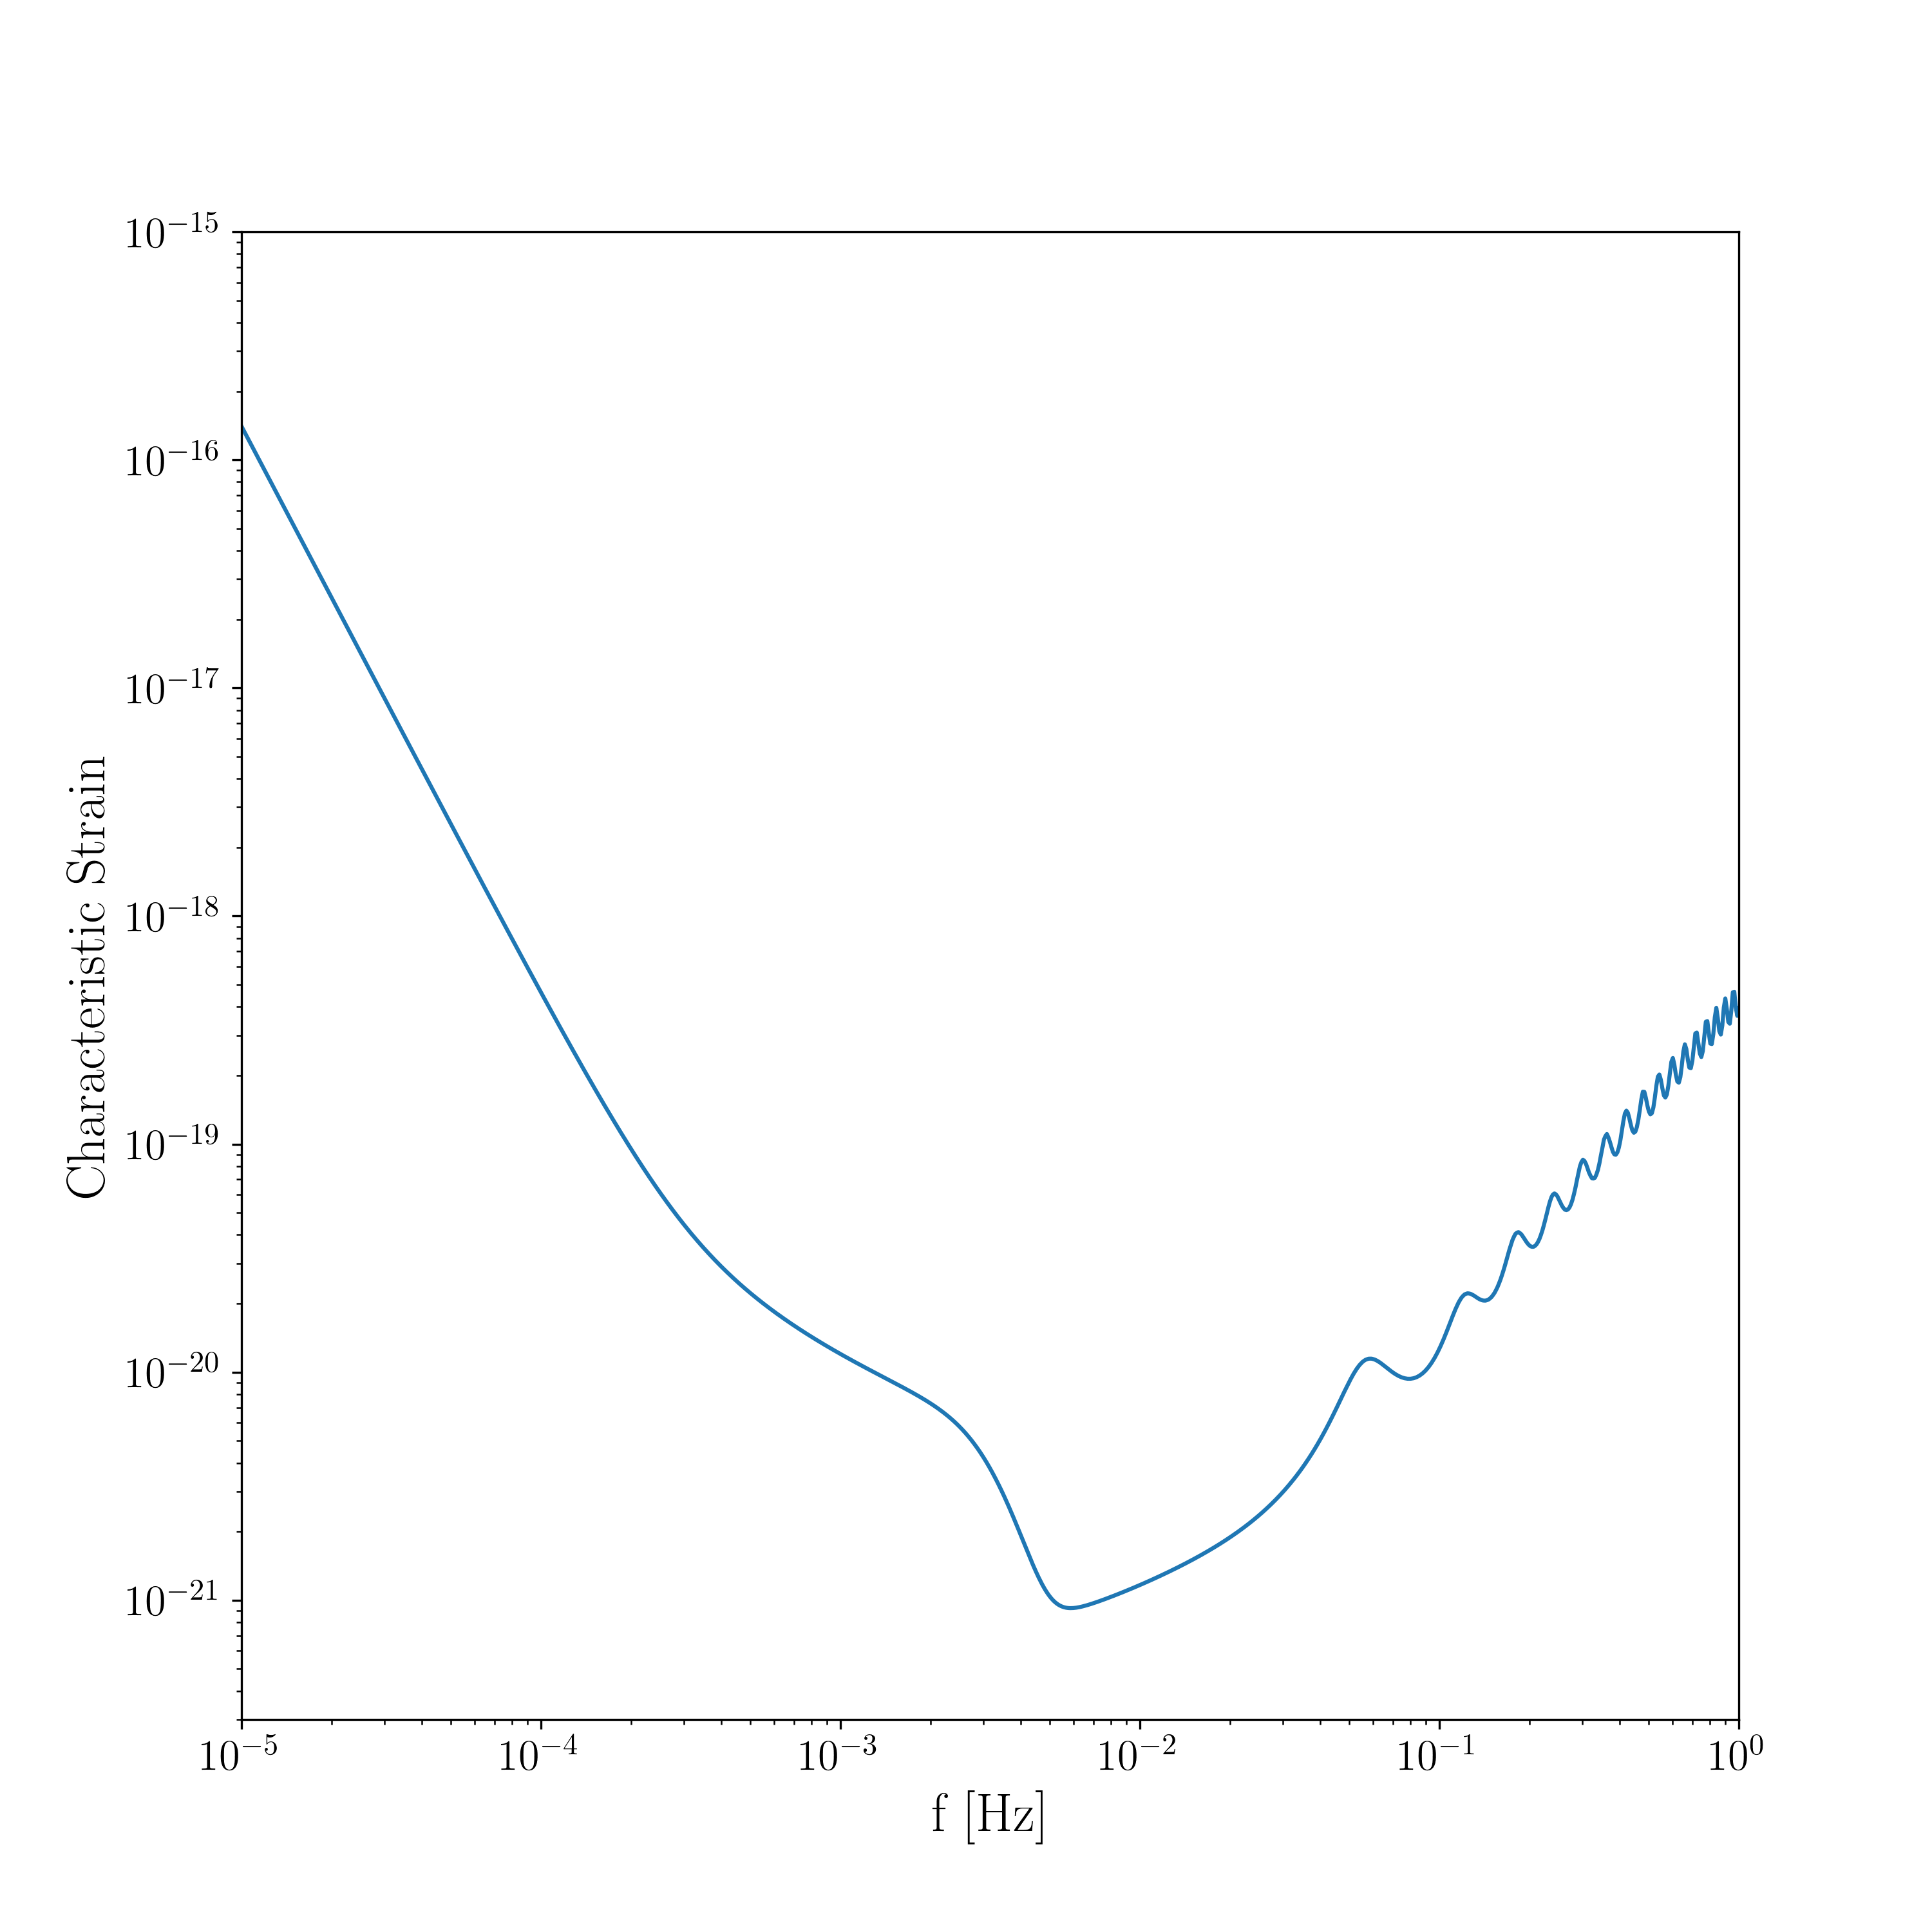
\includegraphics[width=\columnwidth]{LISANoise.png}
%	\caption{The LISA sensitivity curve. Characteristic strain is given by $\sqrt{f (S_n + S_c)}$ }
%	\label{fig:LISA_NOISE}
%\end{figure}









\section{Conclusion}


\newpage
\appendix

%\section{Extra figures}
%\begin{figure*}
%	\subfloat[\label{fig:eg1}]{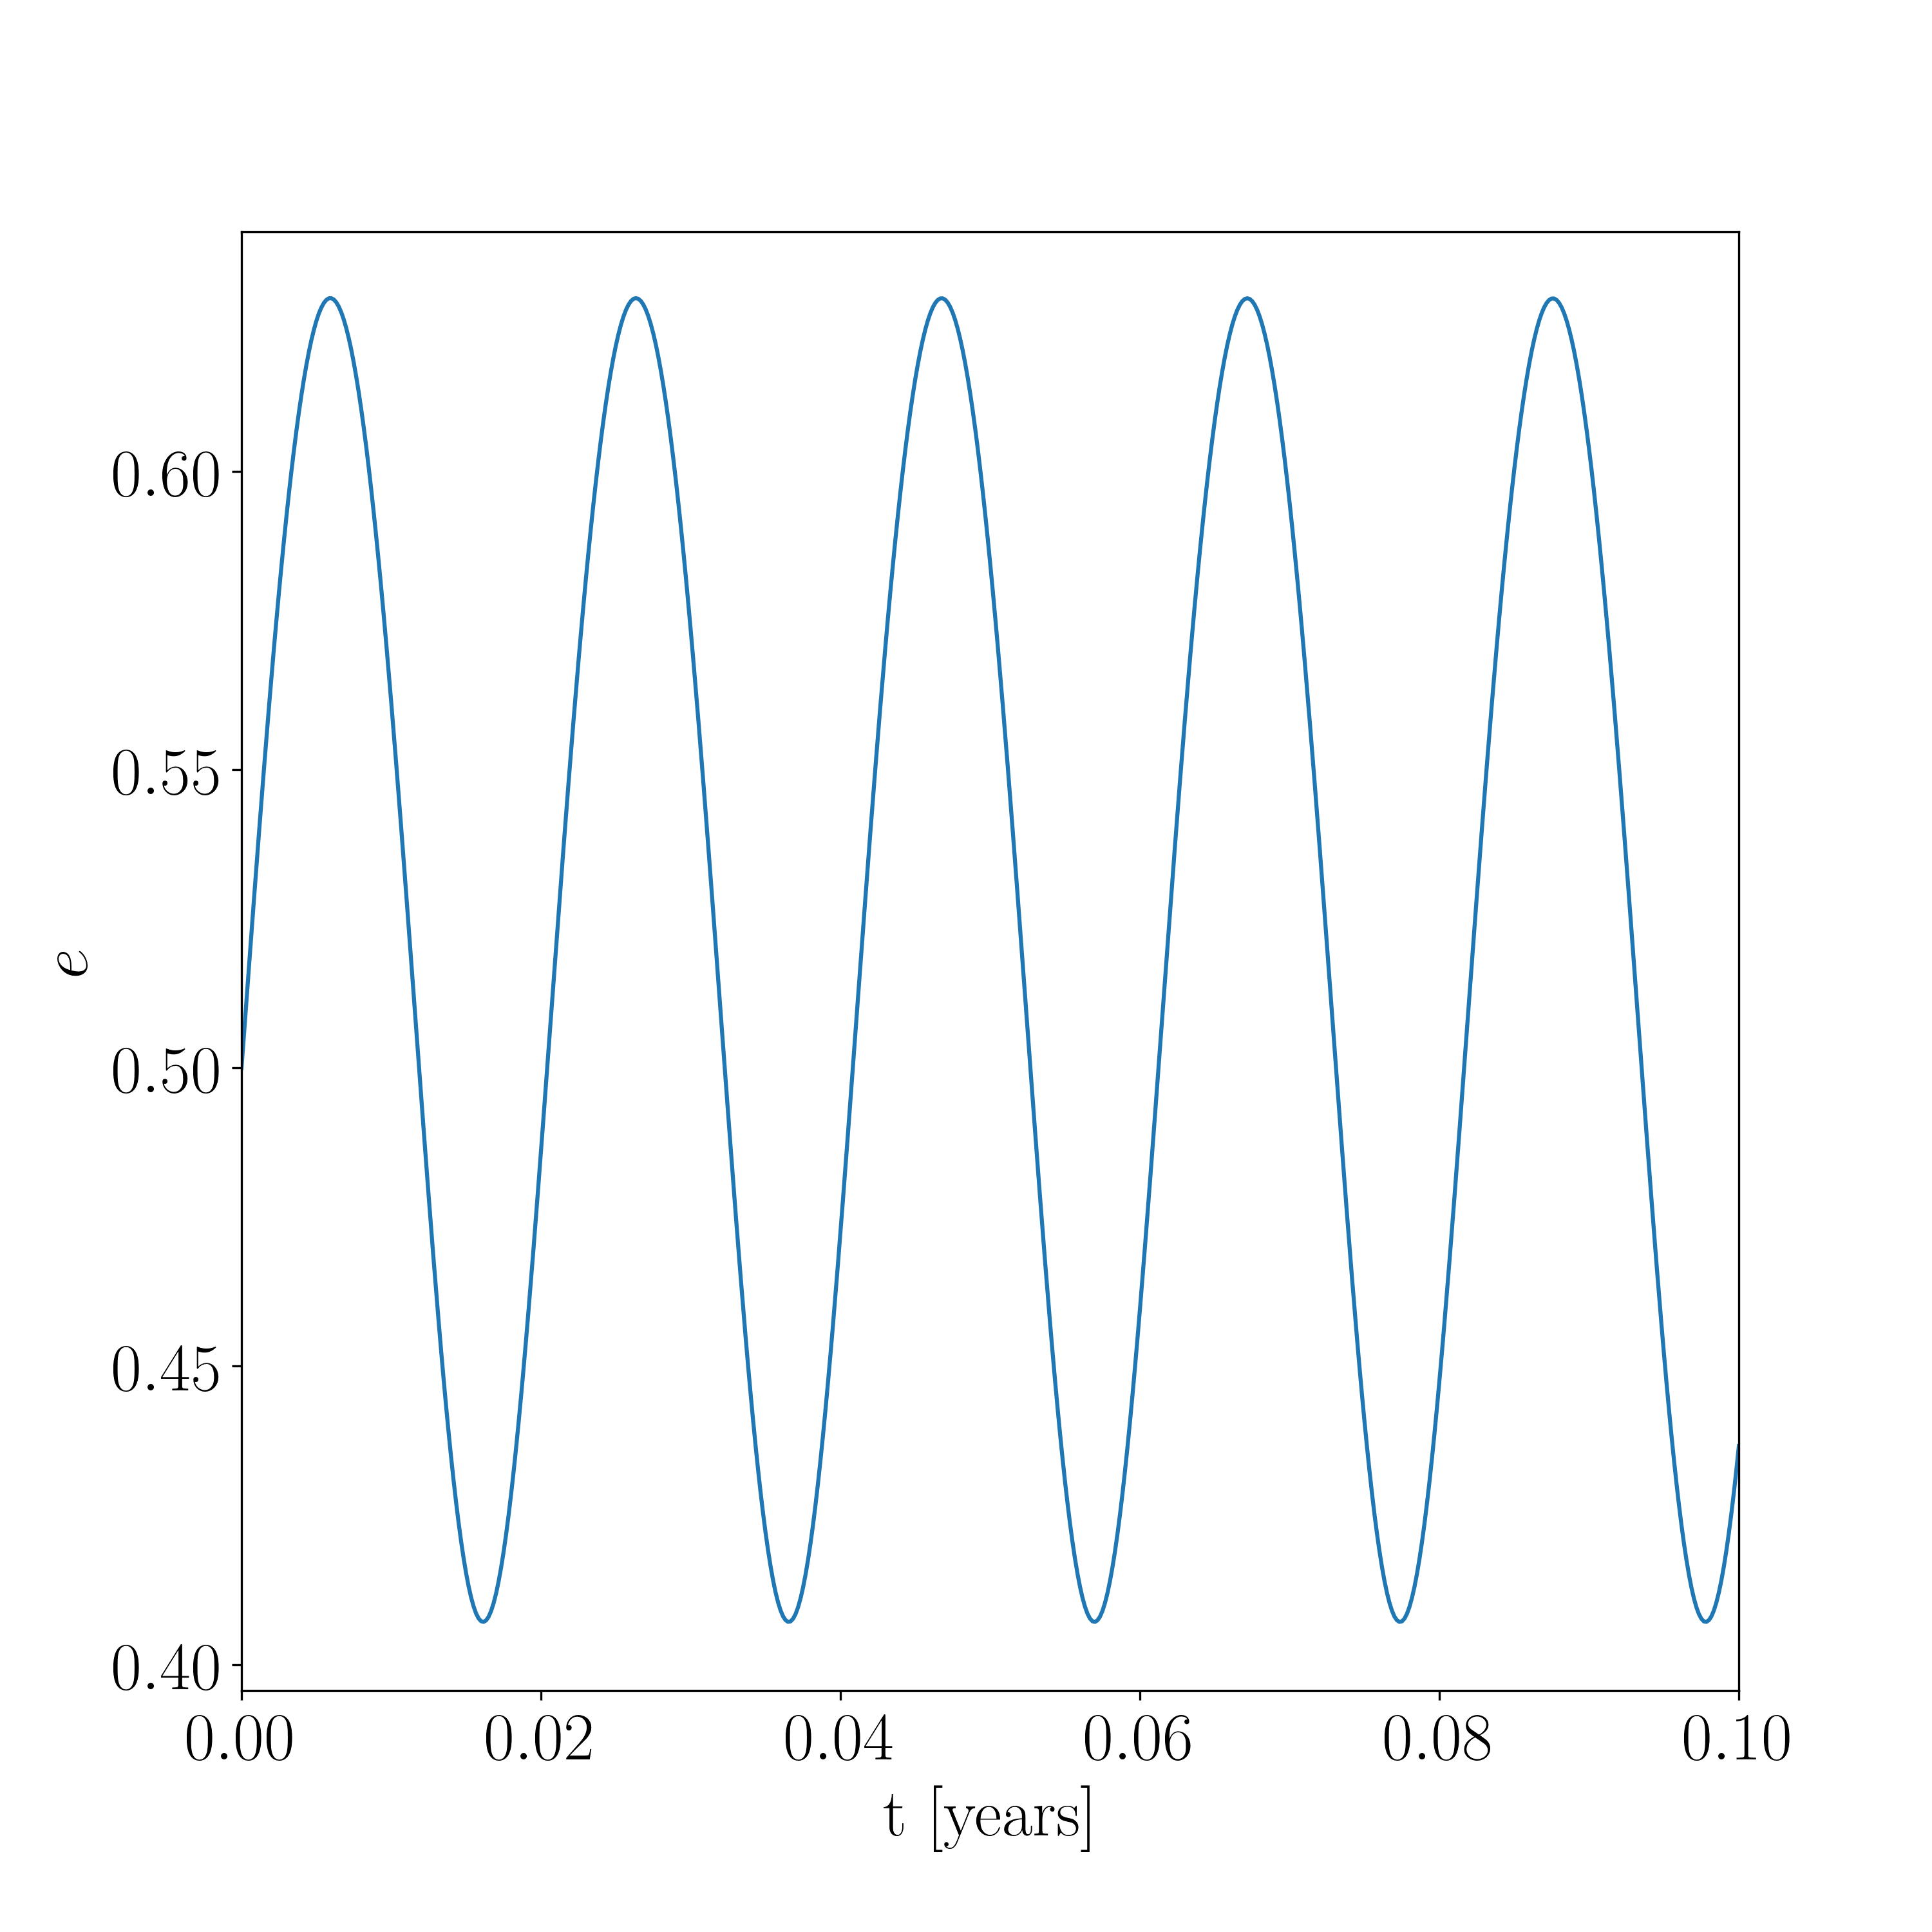
\includegraphics[width=0.48\textwidth]{e_exampleB10.png}}
%	\subfloat[\label{fig:eg2}]{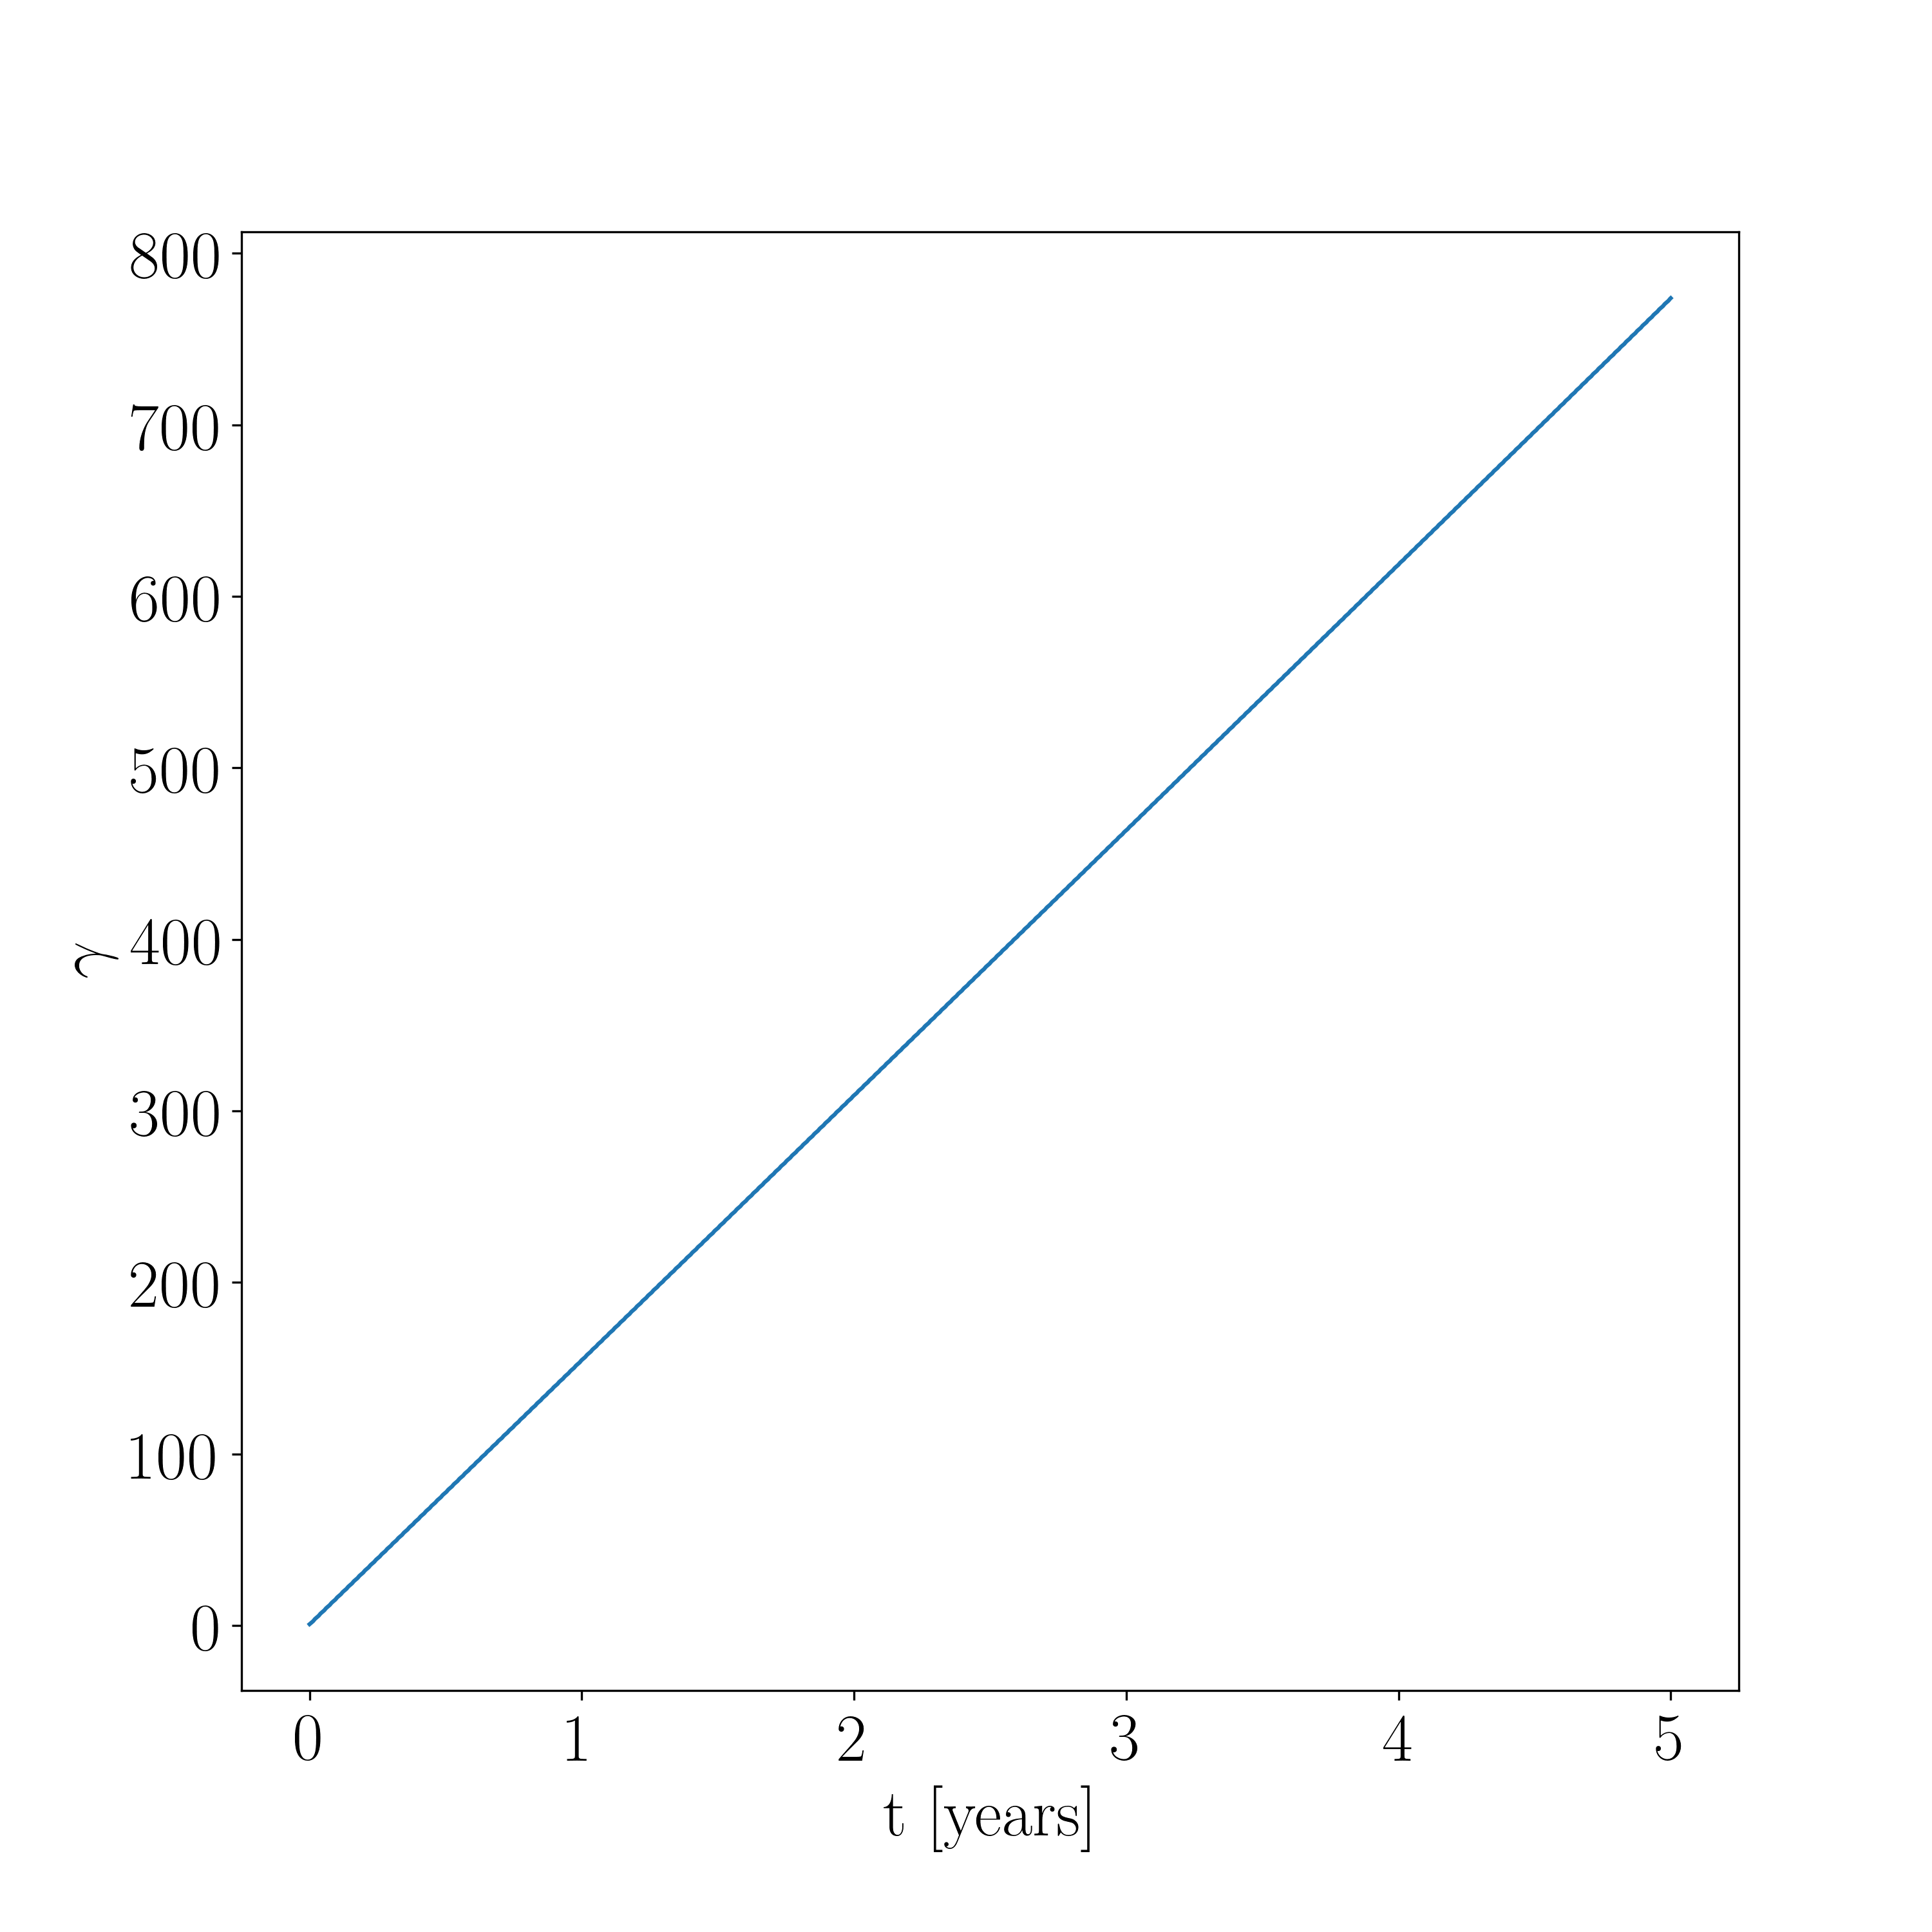
\includegraphics[width=0.48\textwidth]{g_exampleB10.png}} \\
%	\subfloat[\label{fig:eg3}]{\includegraphics[width=0.48\textwidth]{e_exampleB100.png}}
%	\subfloat[\label{fig:eg4}]{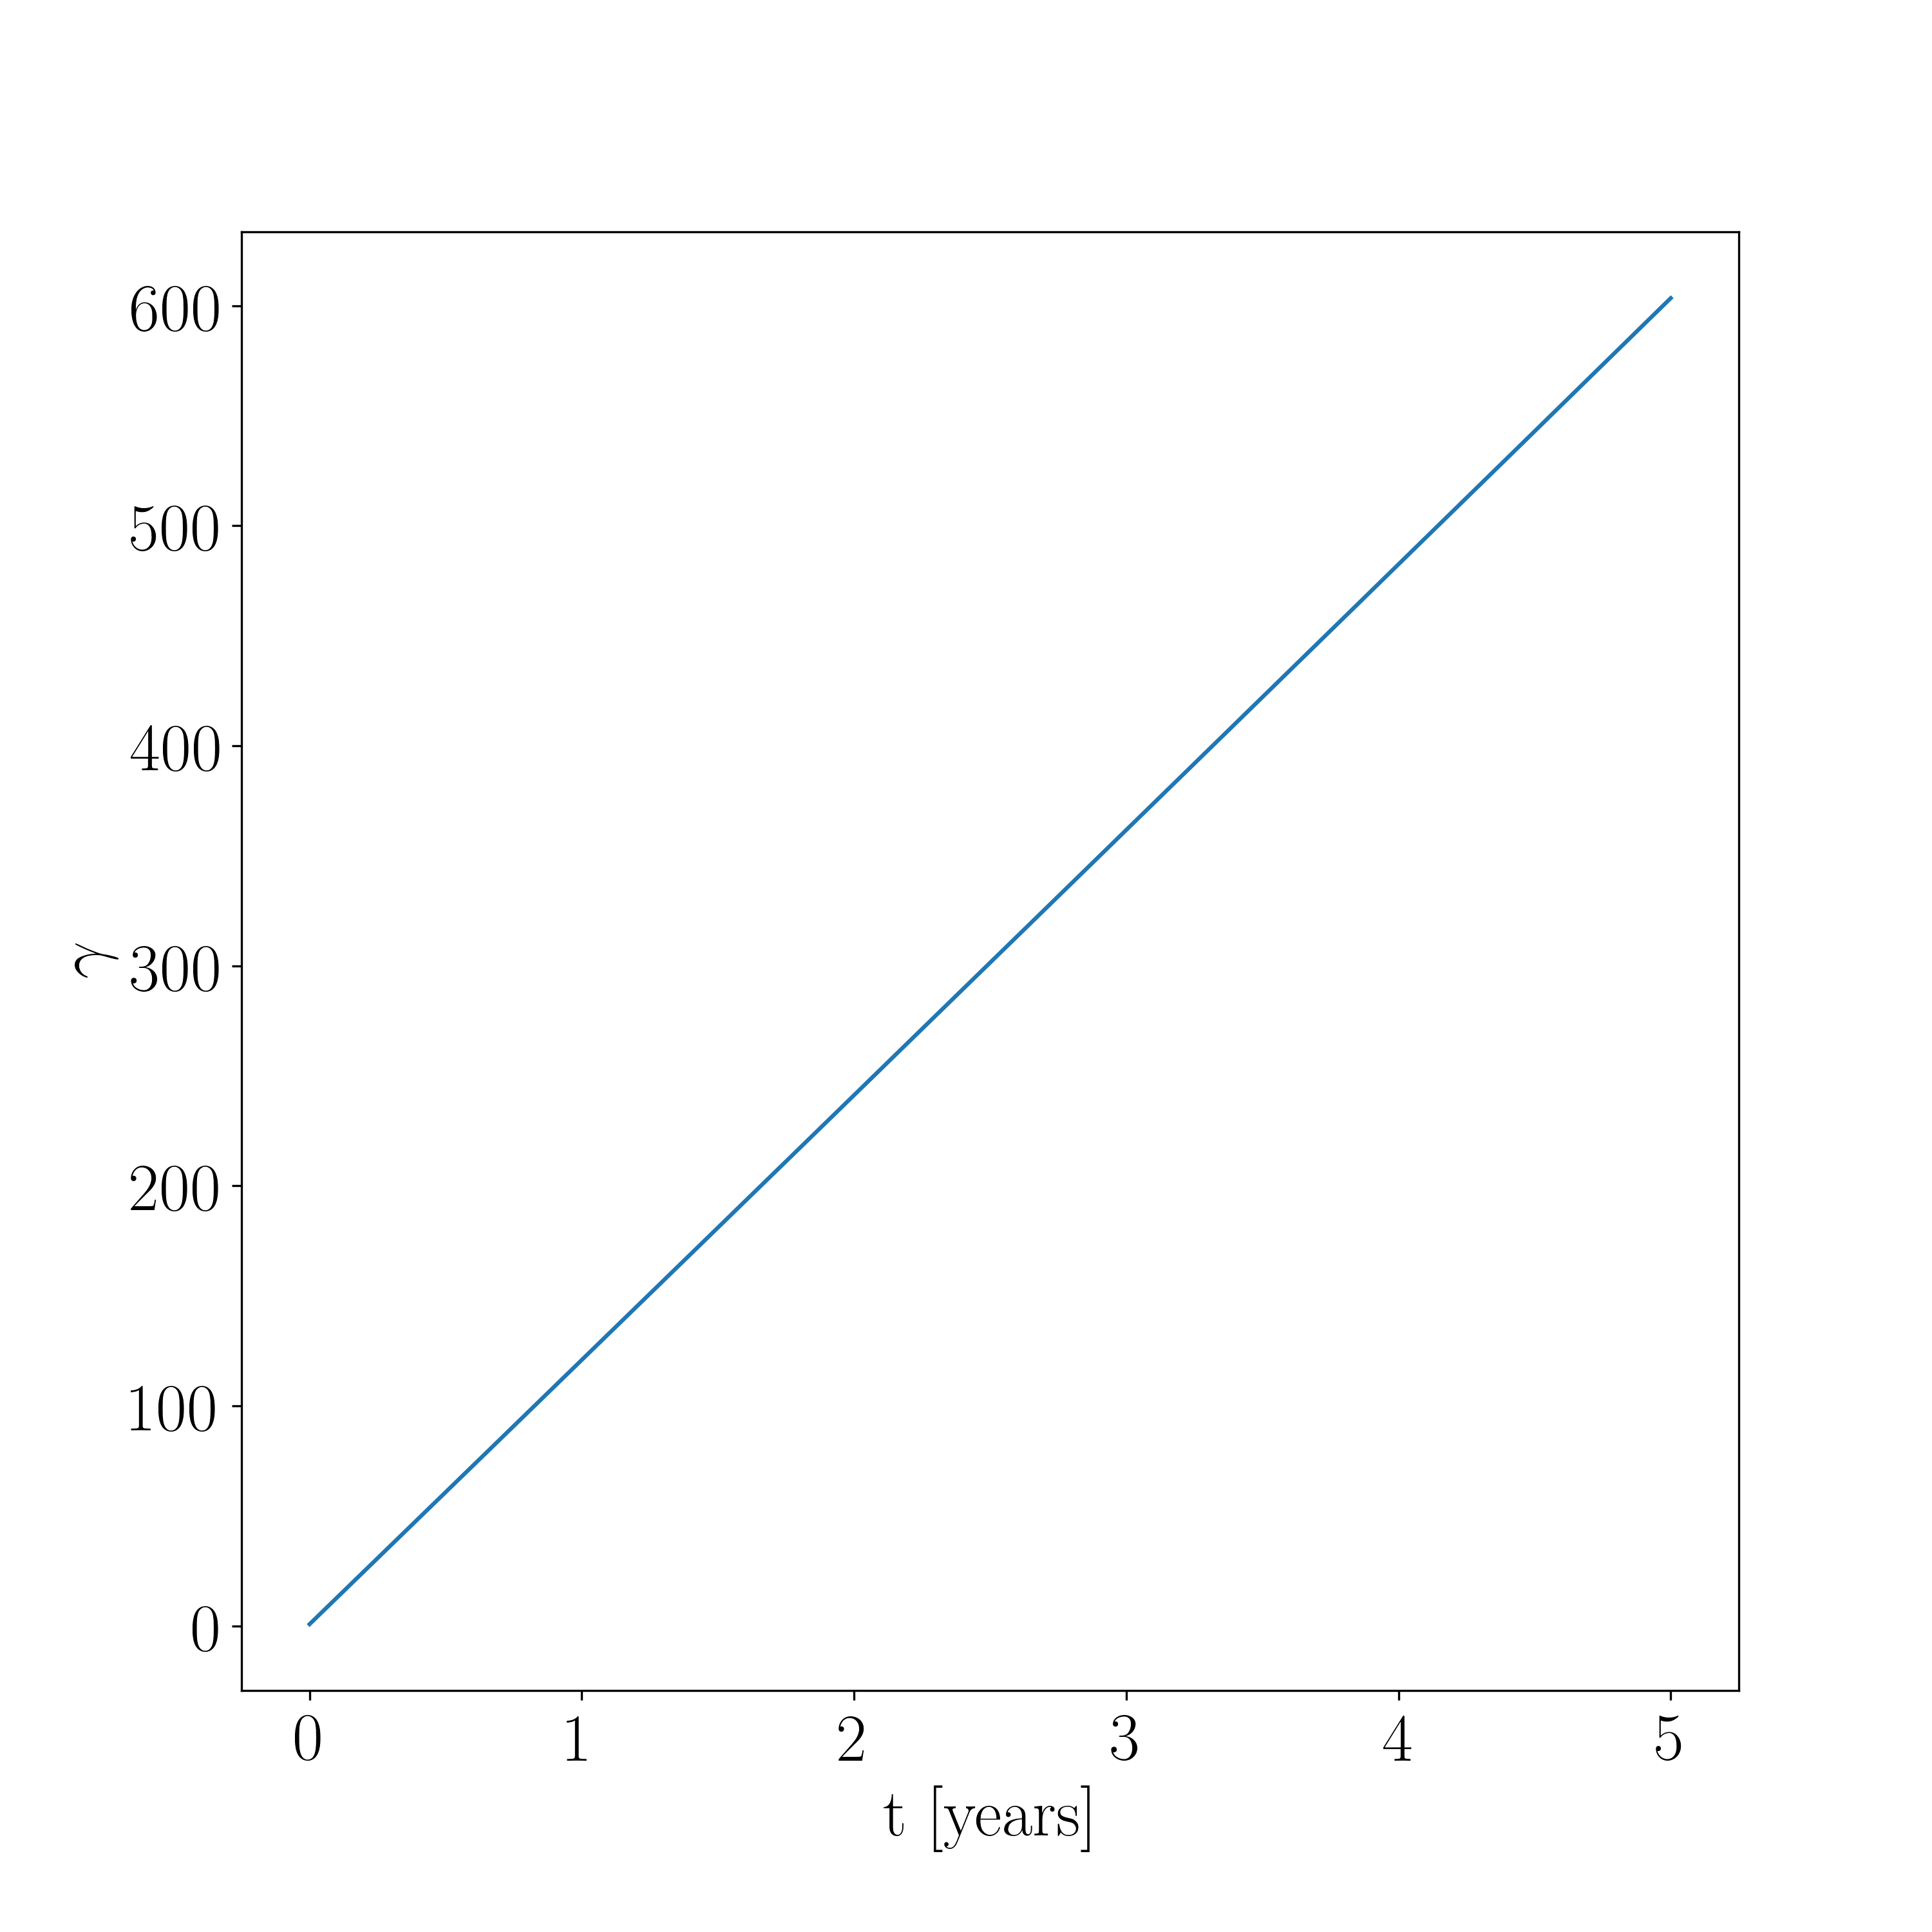
\includegraphics[width=0.48\textwidth]{g_exampleB100.png}} 
%	\caption{\textit{Top row:} Evolution of the eccentricity and pericentre angle on the inner binary in a hierarchical triple with $\beta = 10$, by solving the set of ODEs numerically. \textit{Bottom row:} as top row for $\beta = 100$. Note decrease in amplitude of eccentricity oscillations and linear evolution of $\gamma$} \label{fig:eg_exampleB10}
%\end{figure*}
%
%
%\begin{figure*}
%	\subfloat[\label{}]{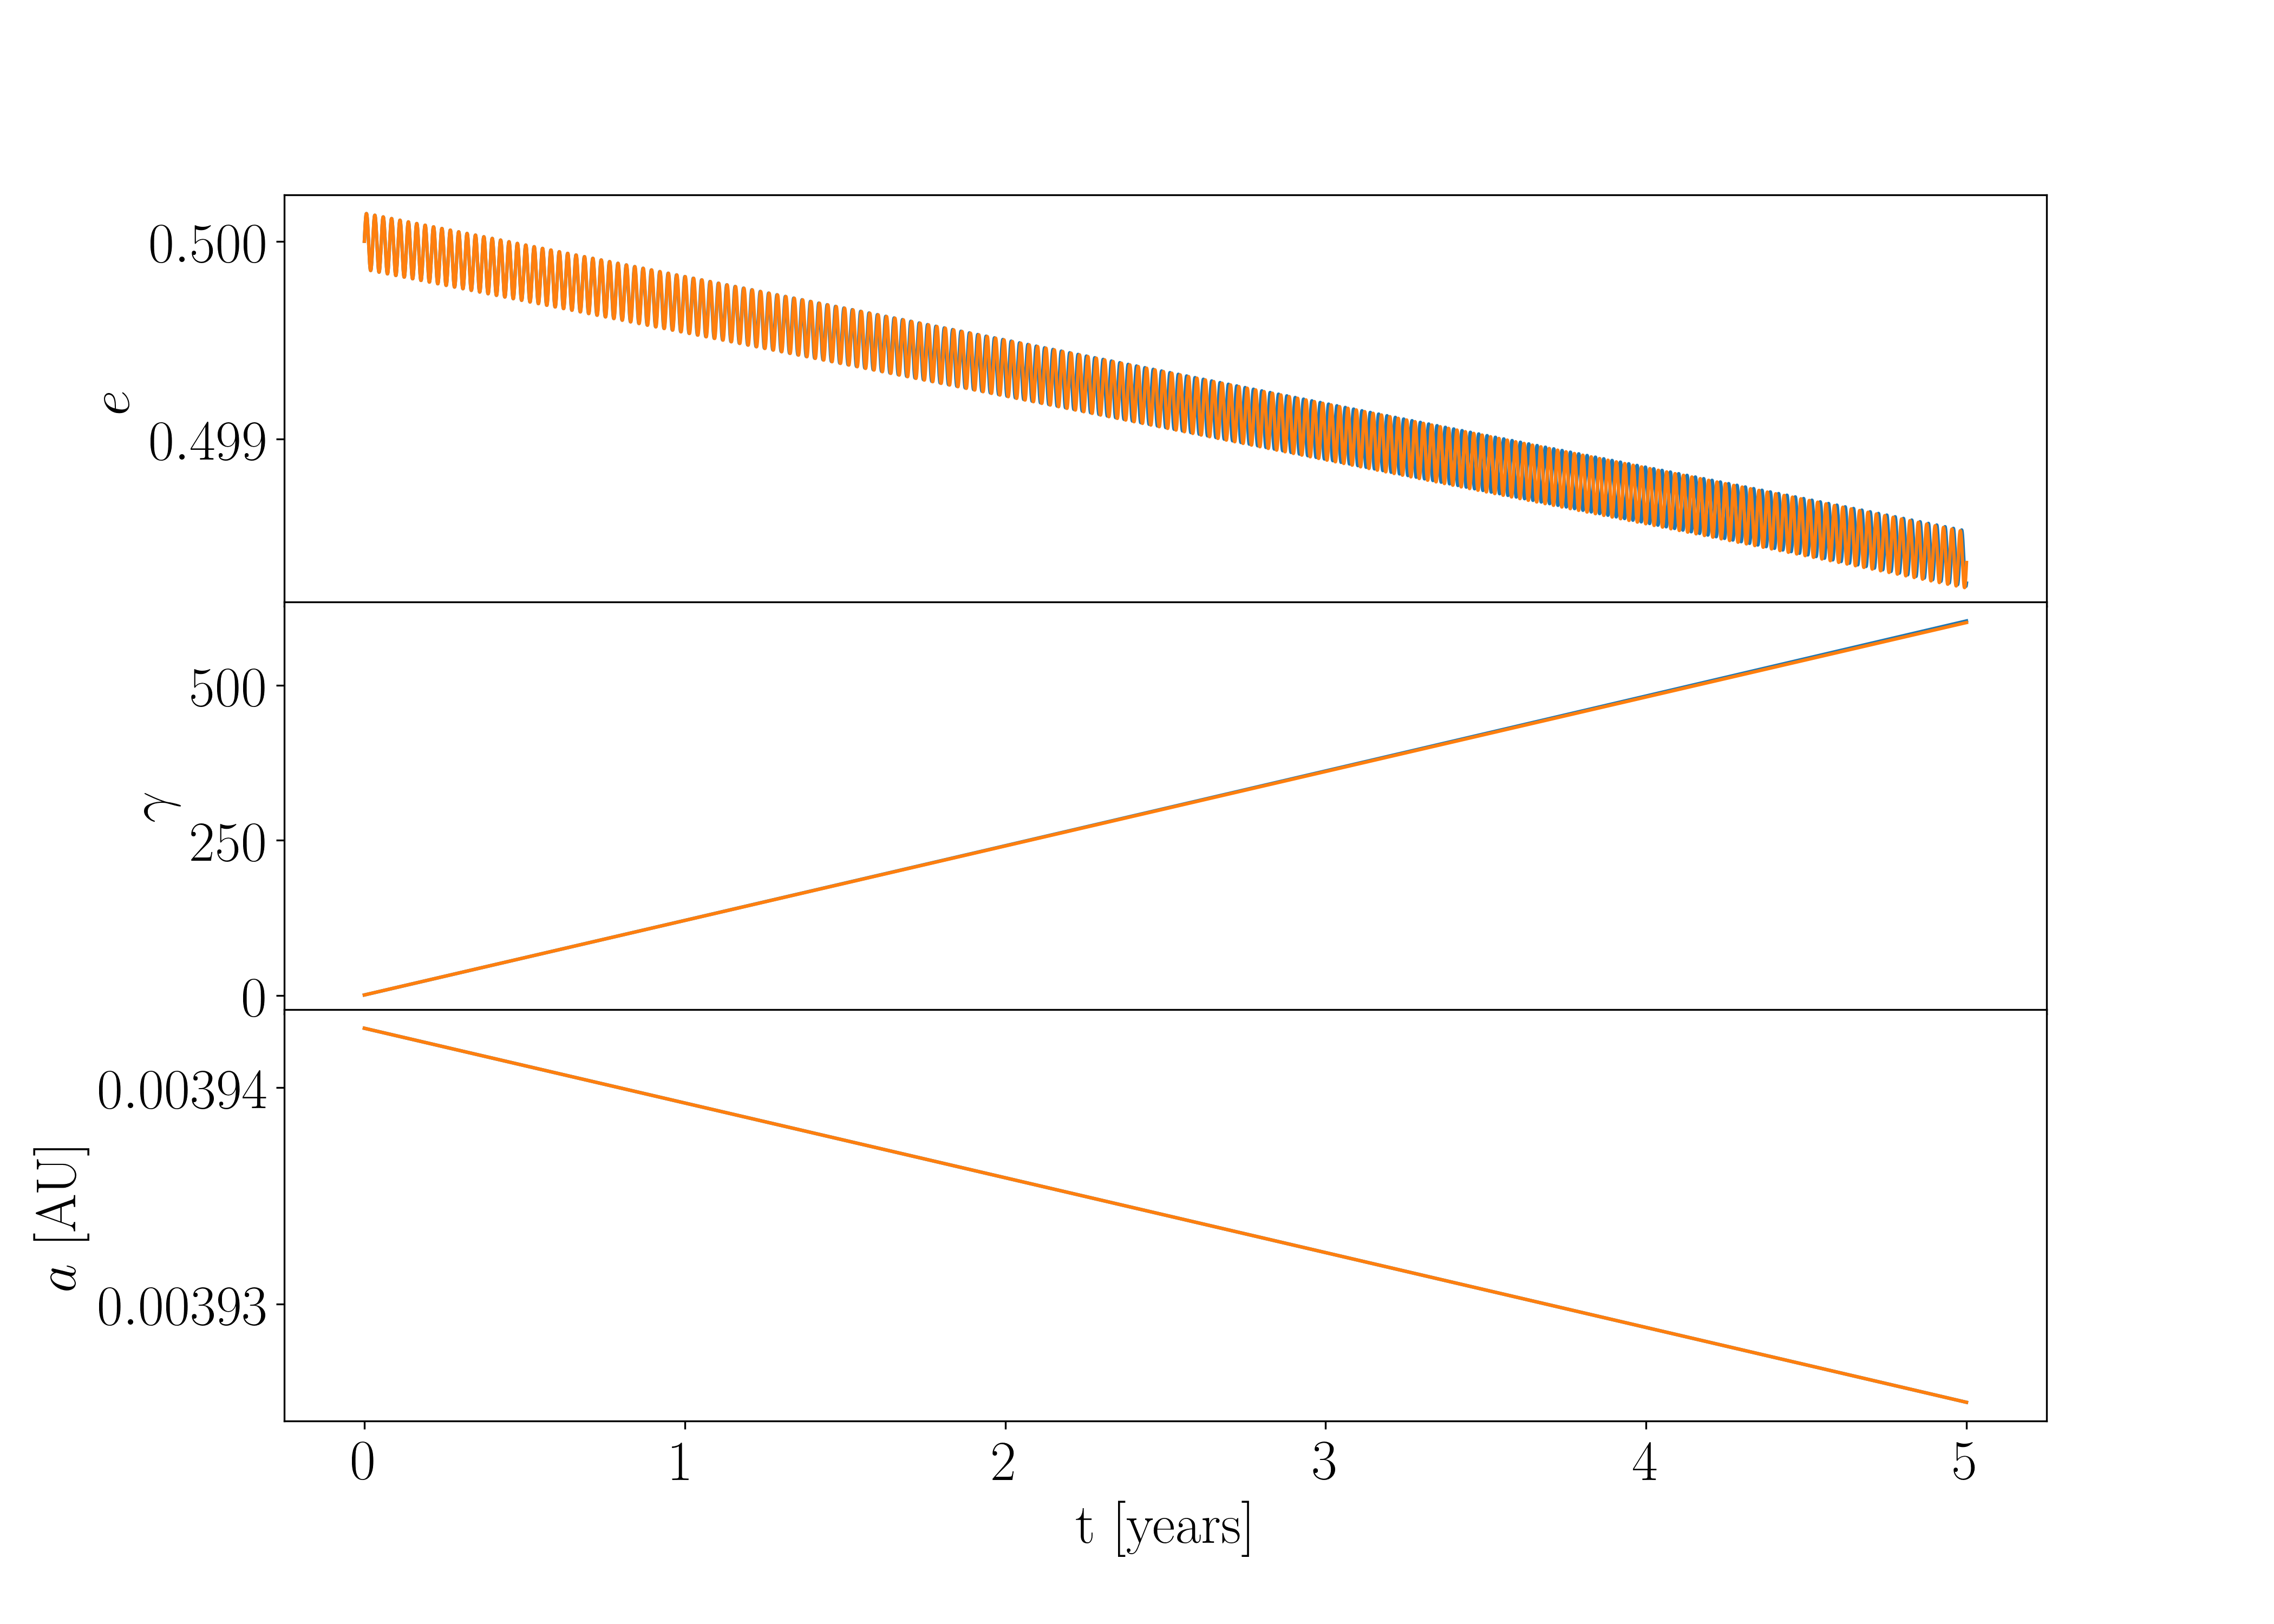
\includegraphics[width=0.8\textwidth]{compare100.png}} \\
%	\subfloat[\label{}]{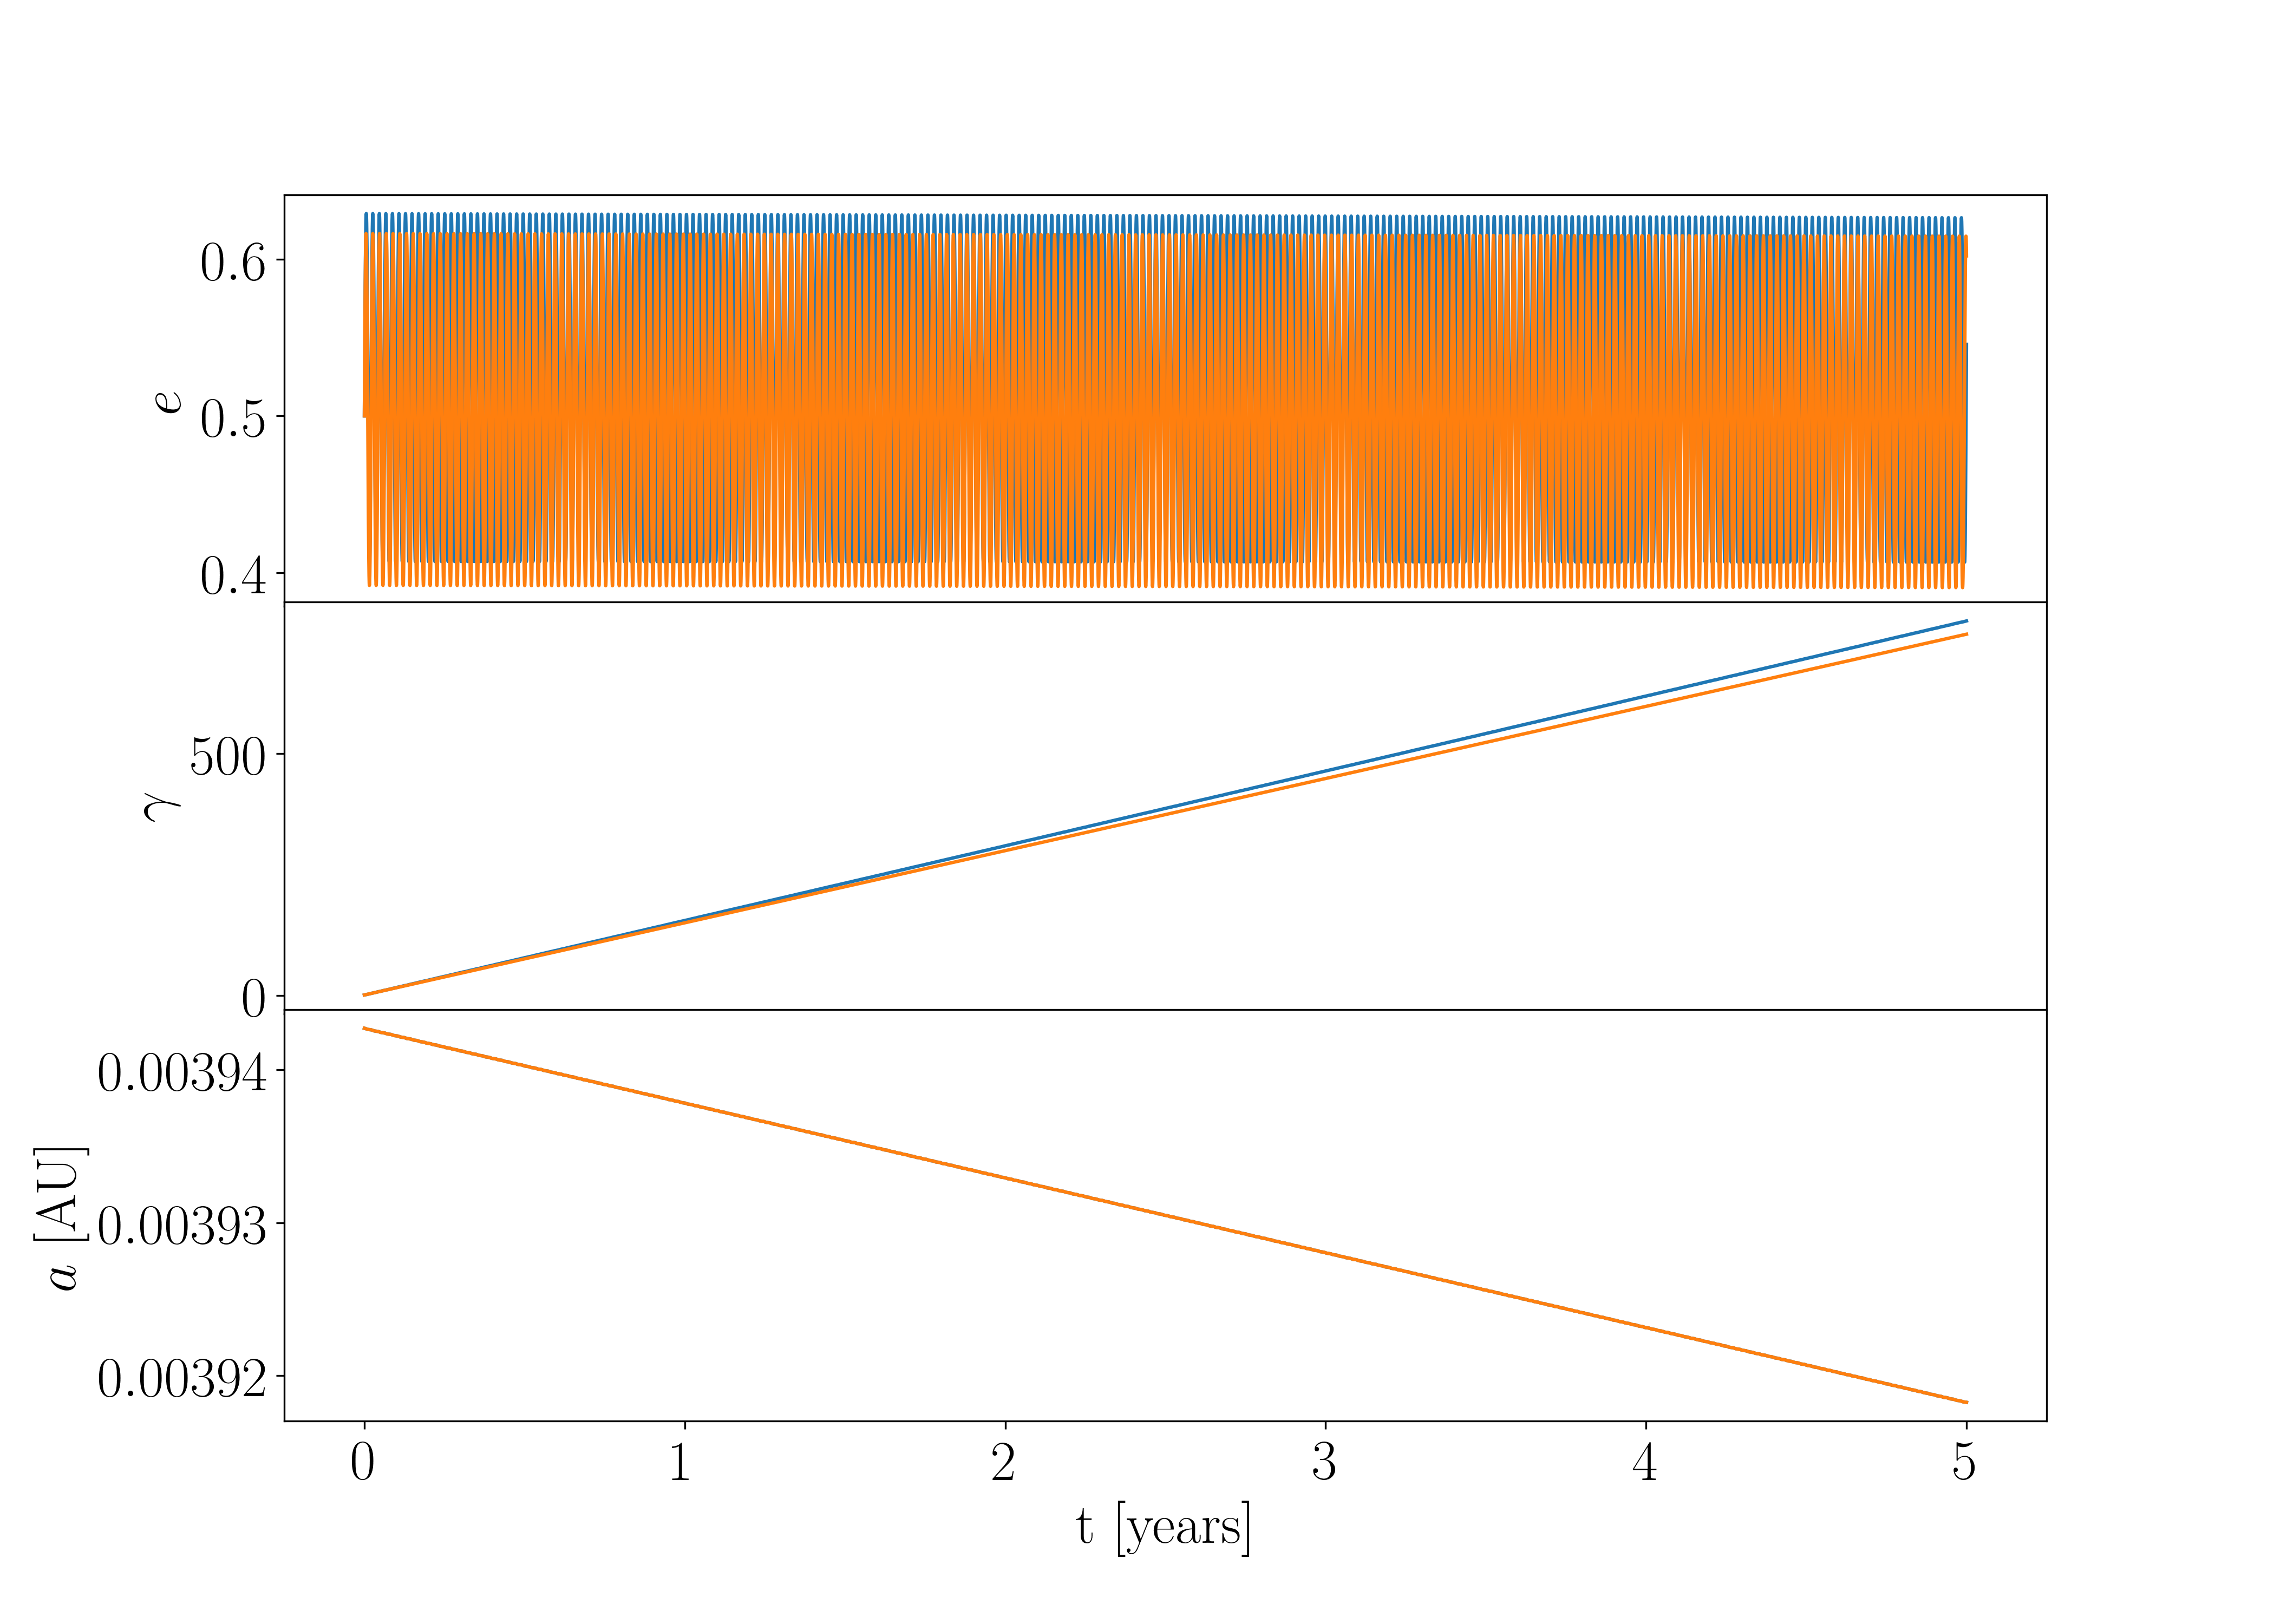
\includegraphics[width=0.8\textwidth]{compare10.png}} \\
%	\medskip
%	\caption{Evolution of $e(t), \gamma(t), a(t)$ for \textit{(a) }$\beta = 100$ and \textit{(b)} $\beta = 10$}
%	\label{fig:spinprecession2}
%\end{figure*}
%
%\begin{figure*}
%	\subfloat[\label{}]{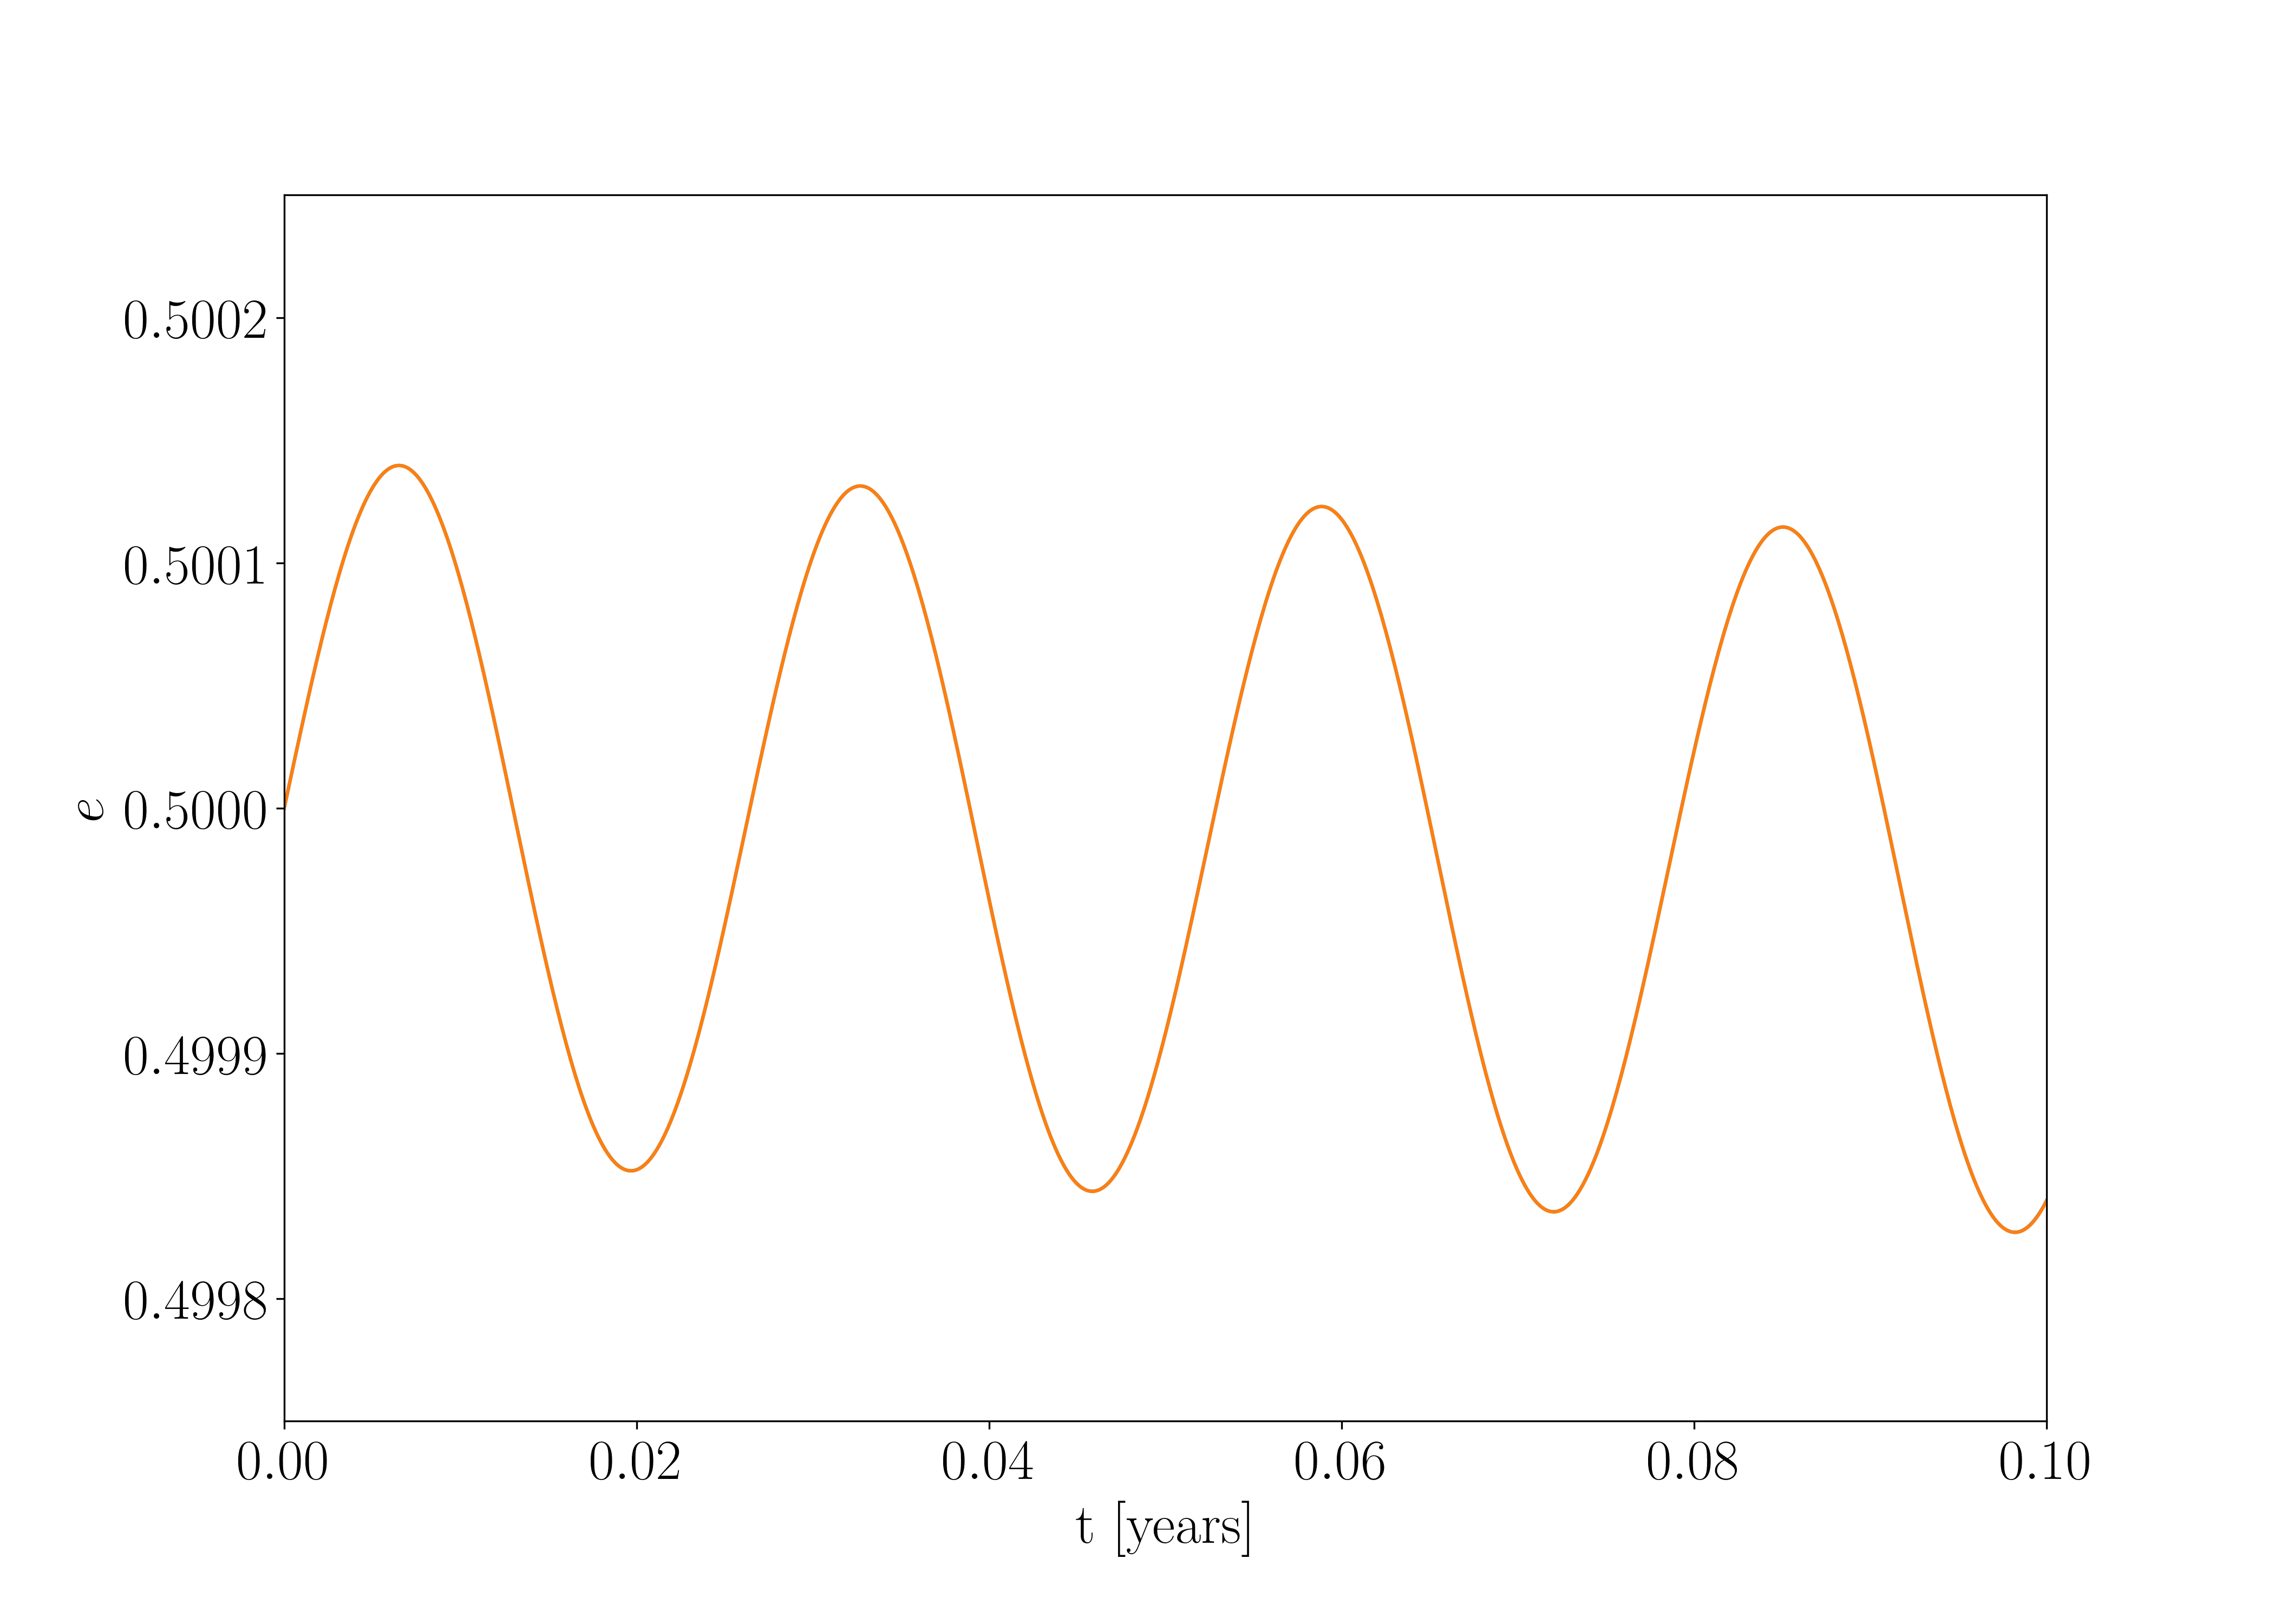
\includegraphics[width=0.7\textwidth]{just_e100.png}} \\ 
%	\subfloat[\label{}]{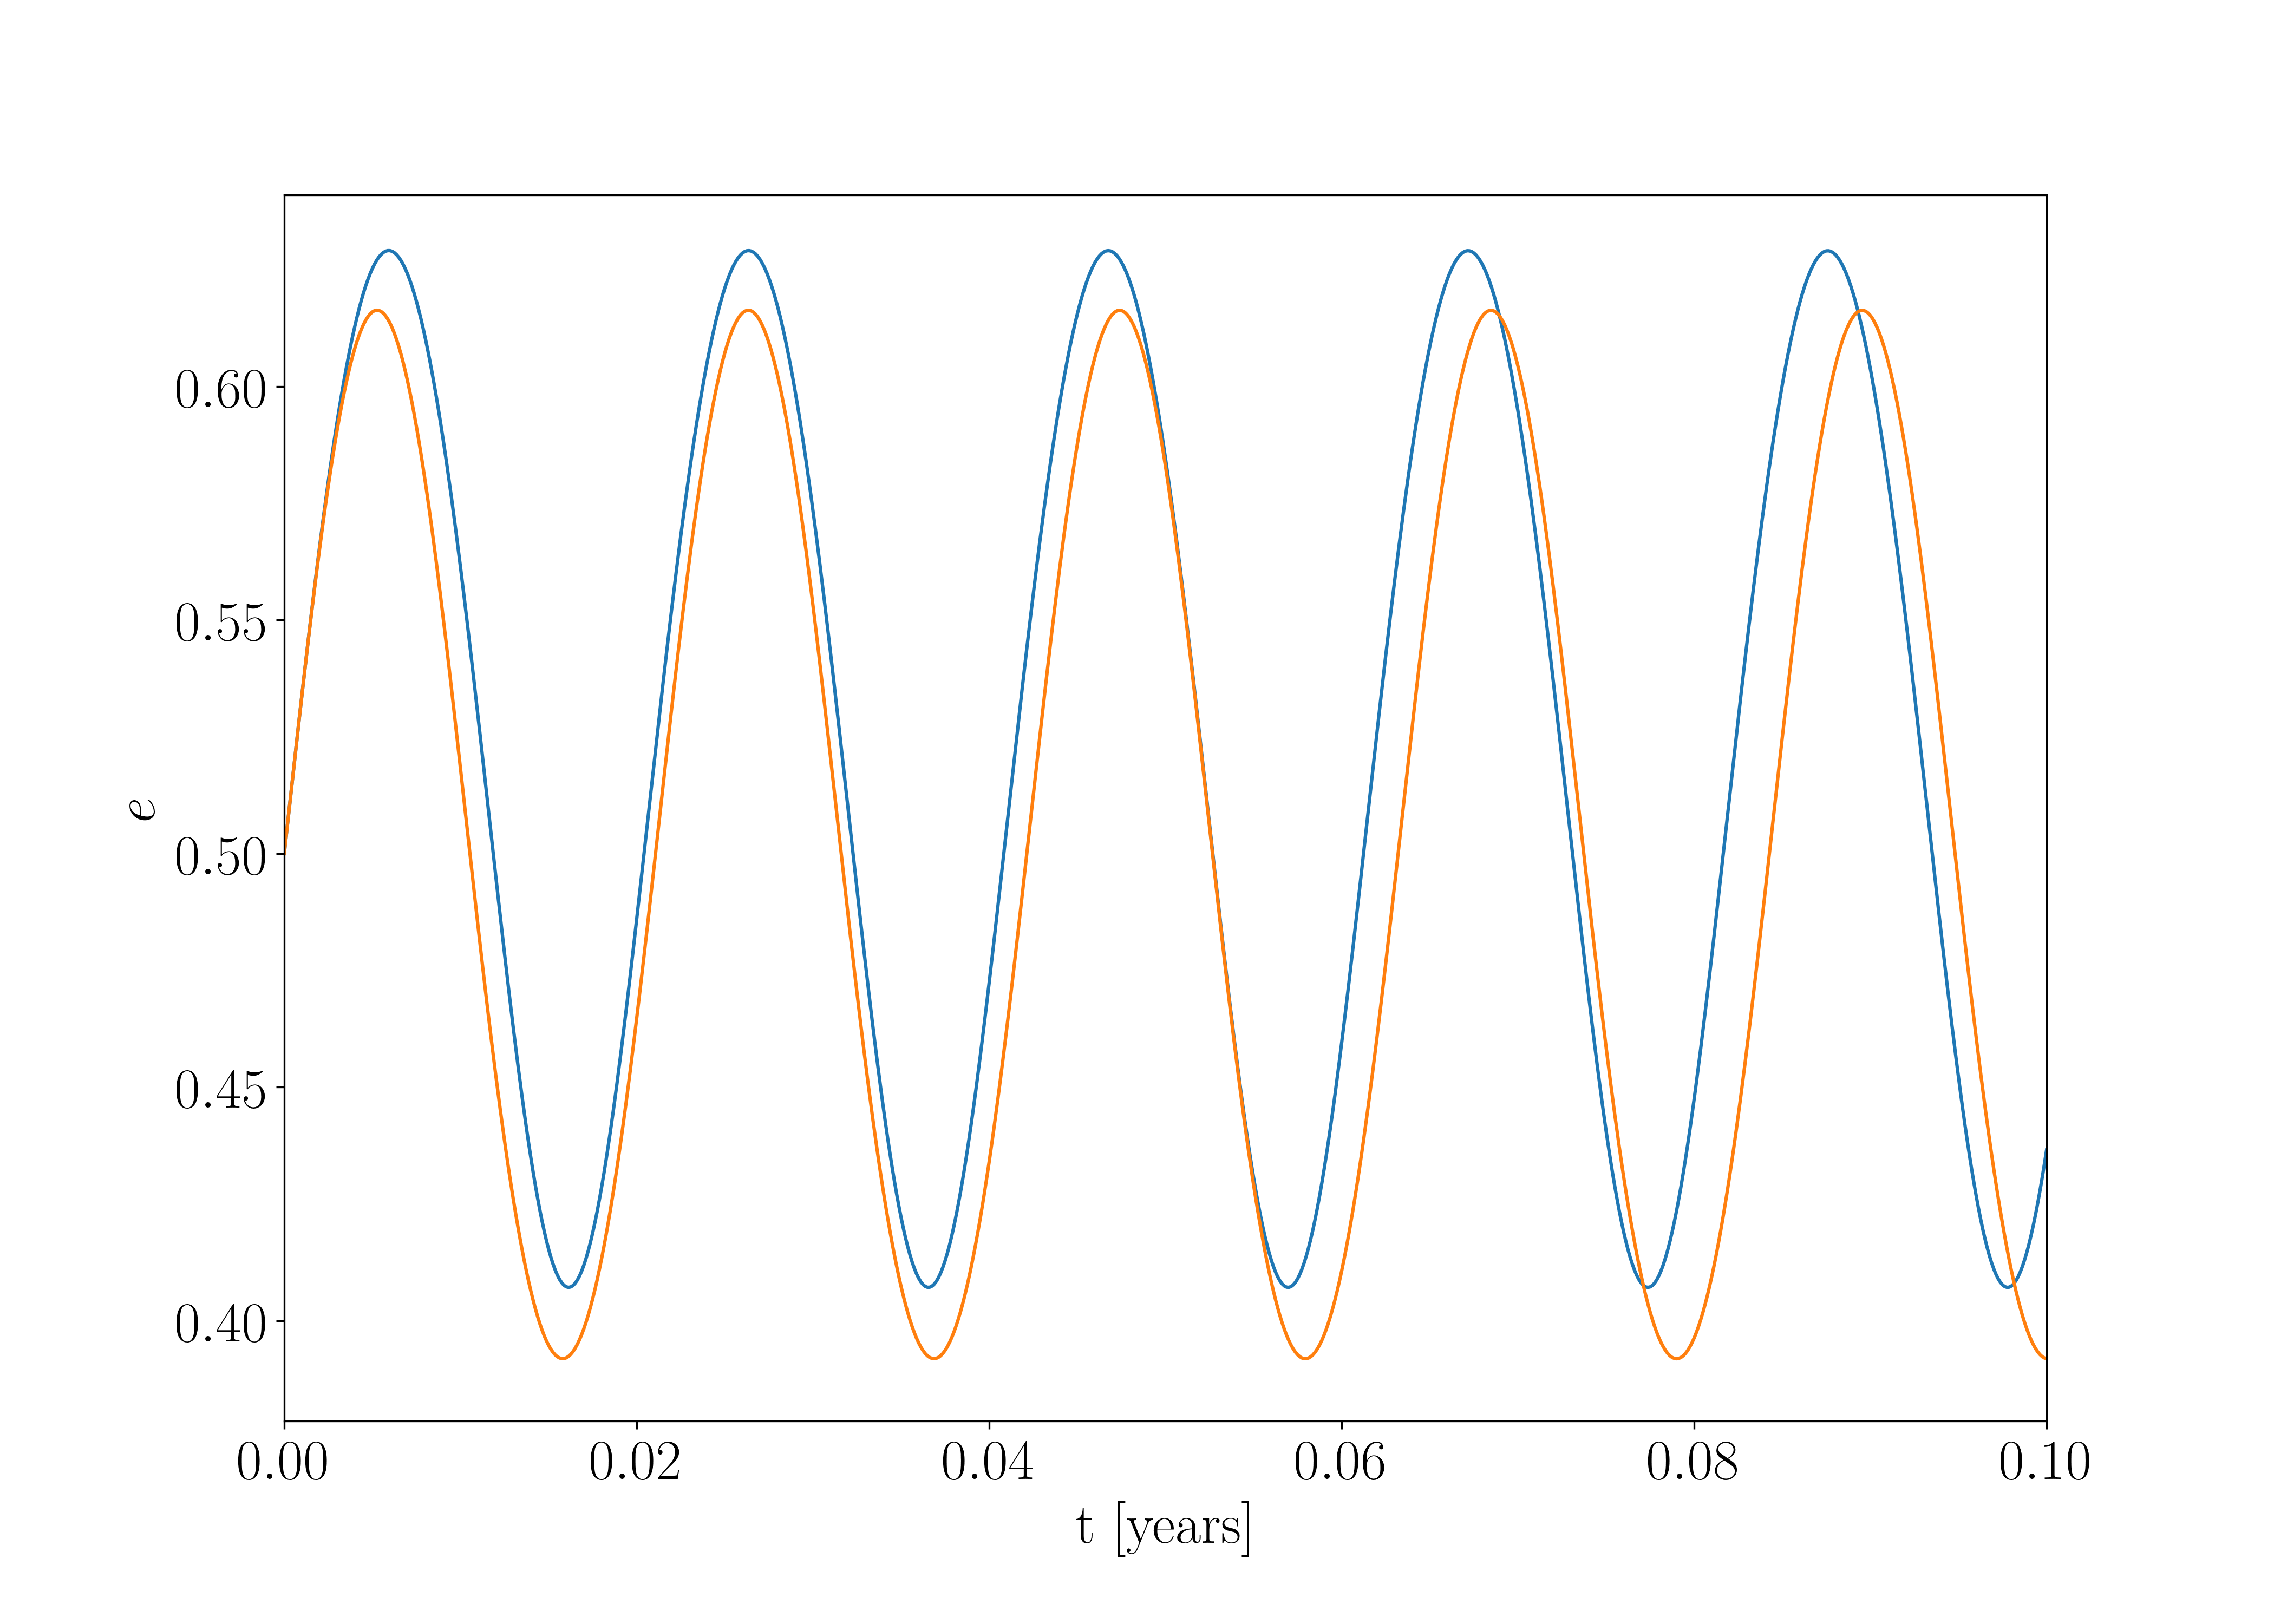
\includegraphics[width=0.7\textwidth]{just_e10.png}}  \\
%	\medskip
%	\caption{As Fig. \ref{fig:spinprecession2} on shorter timescales}
%	\label{fig:comparision2}
%\end{figure*}
%
%
%\begin{figure*}
%	\subfloat[\label{}]{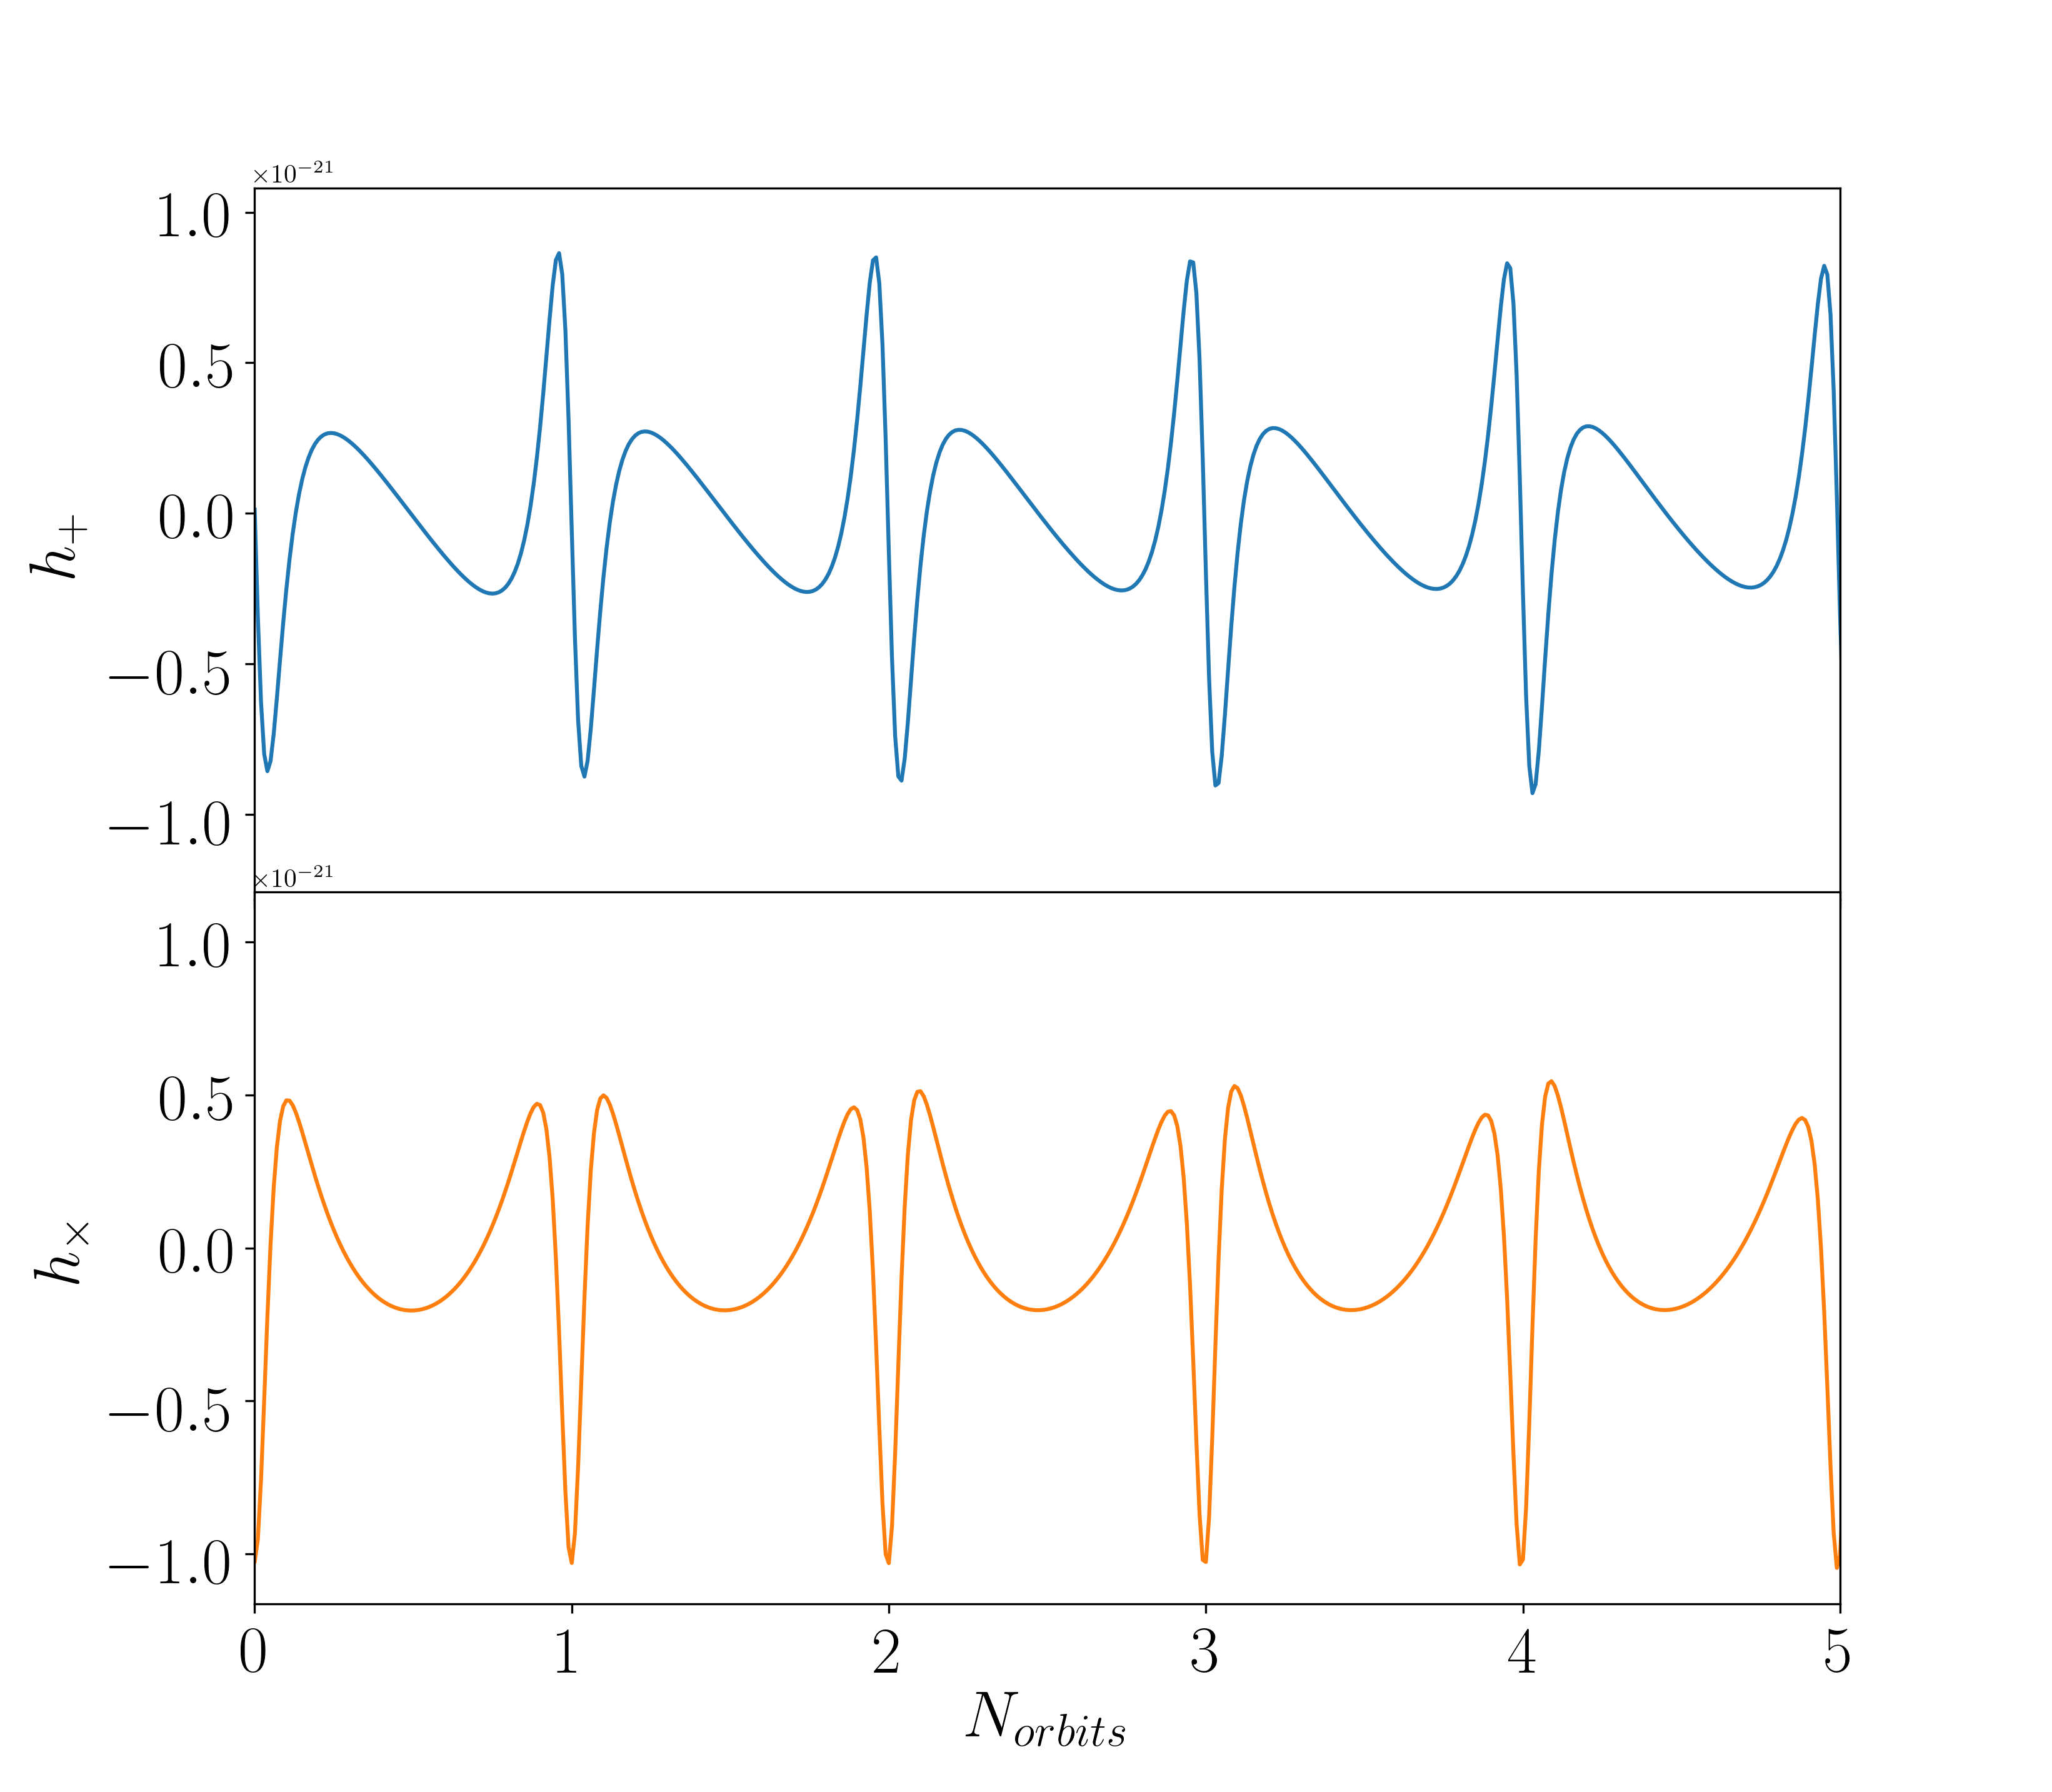
\includegraphics[width=0.8\textwidth]{GW_WaveformsSHORT.png}} \\
%	\subfloat[\label{}]{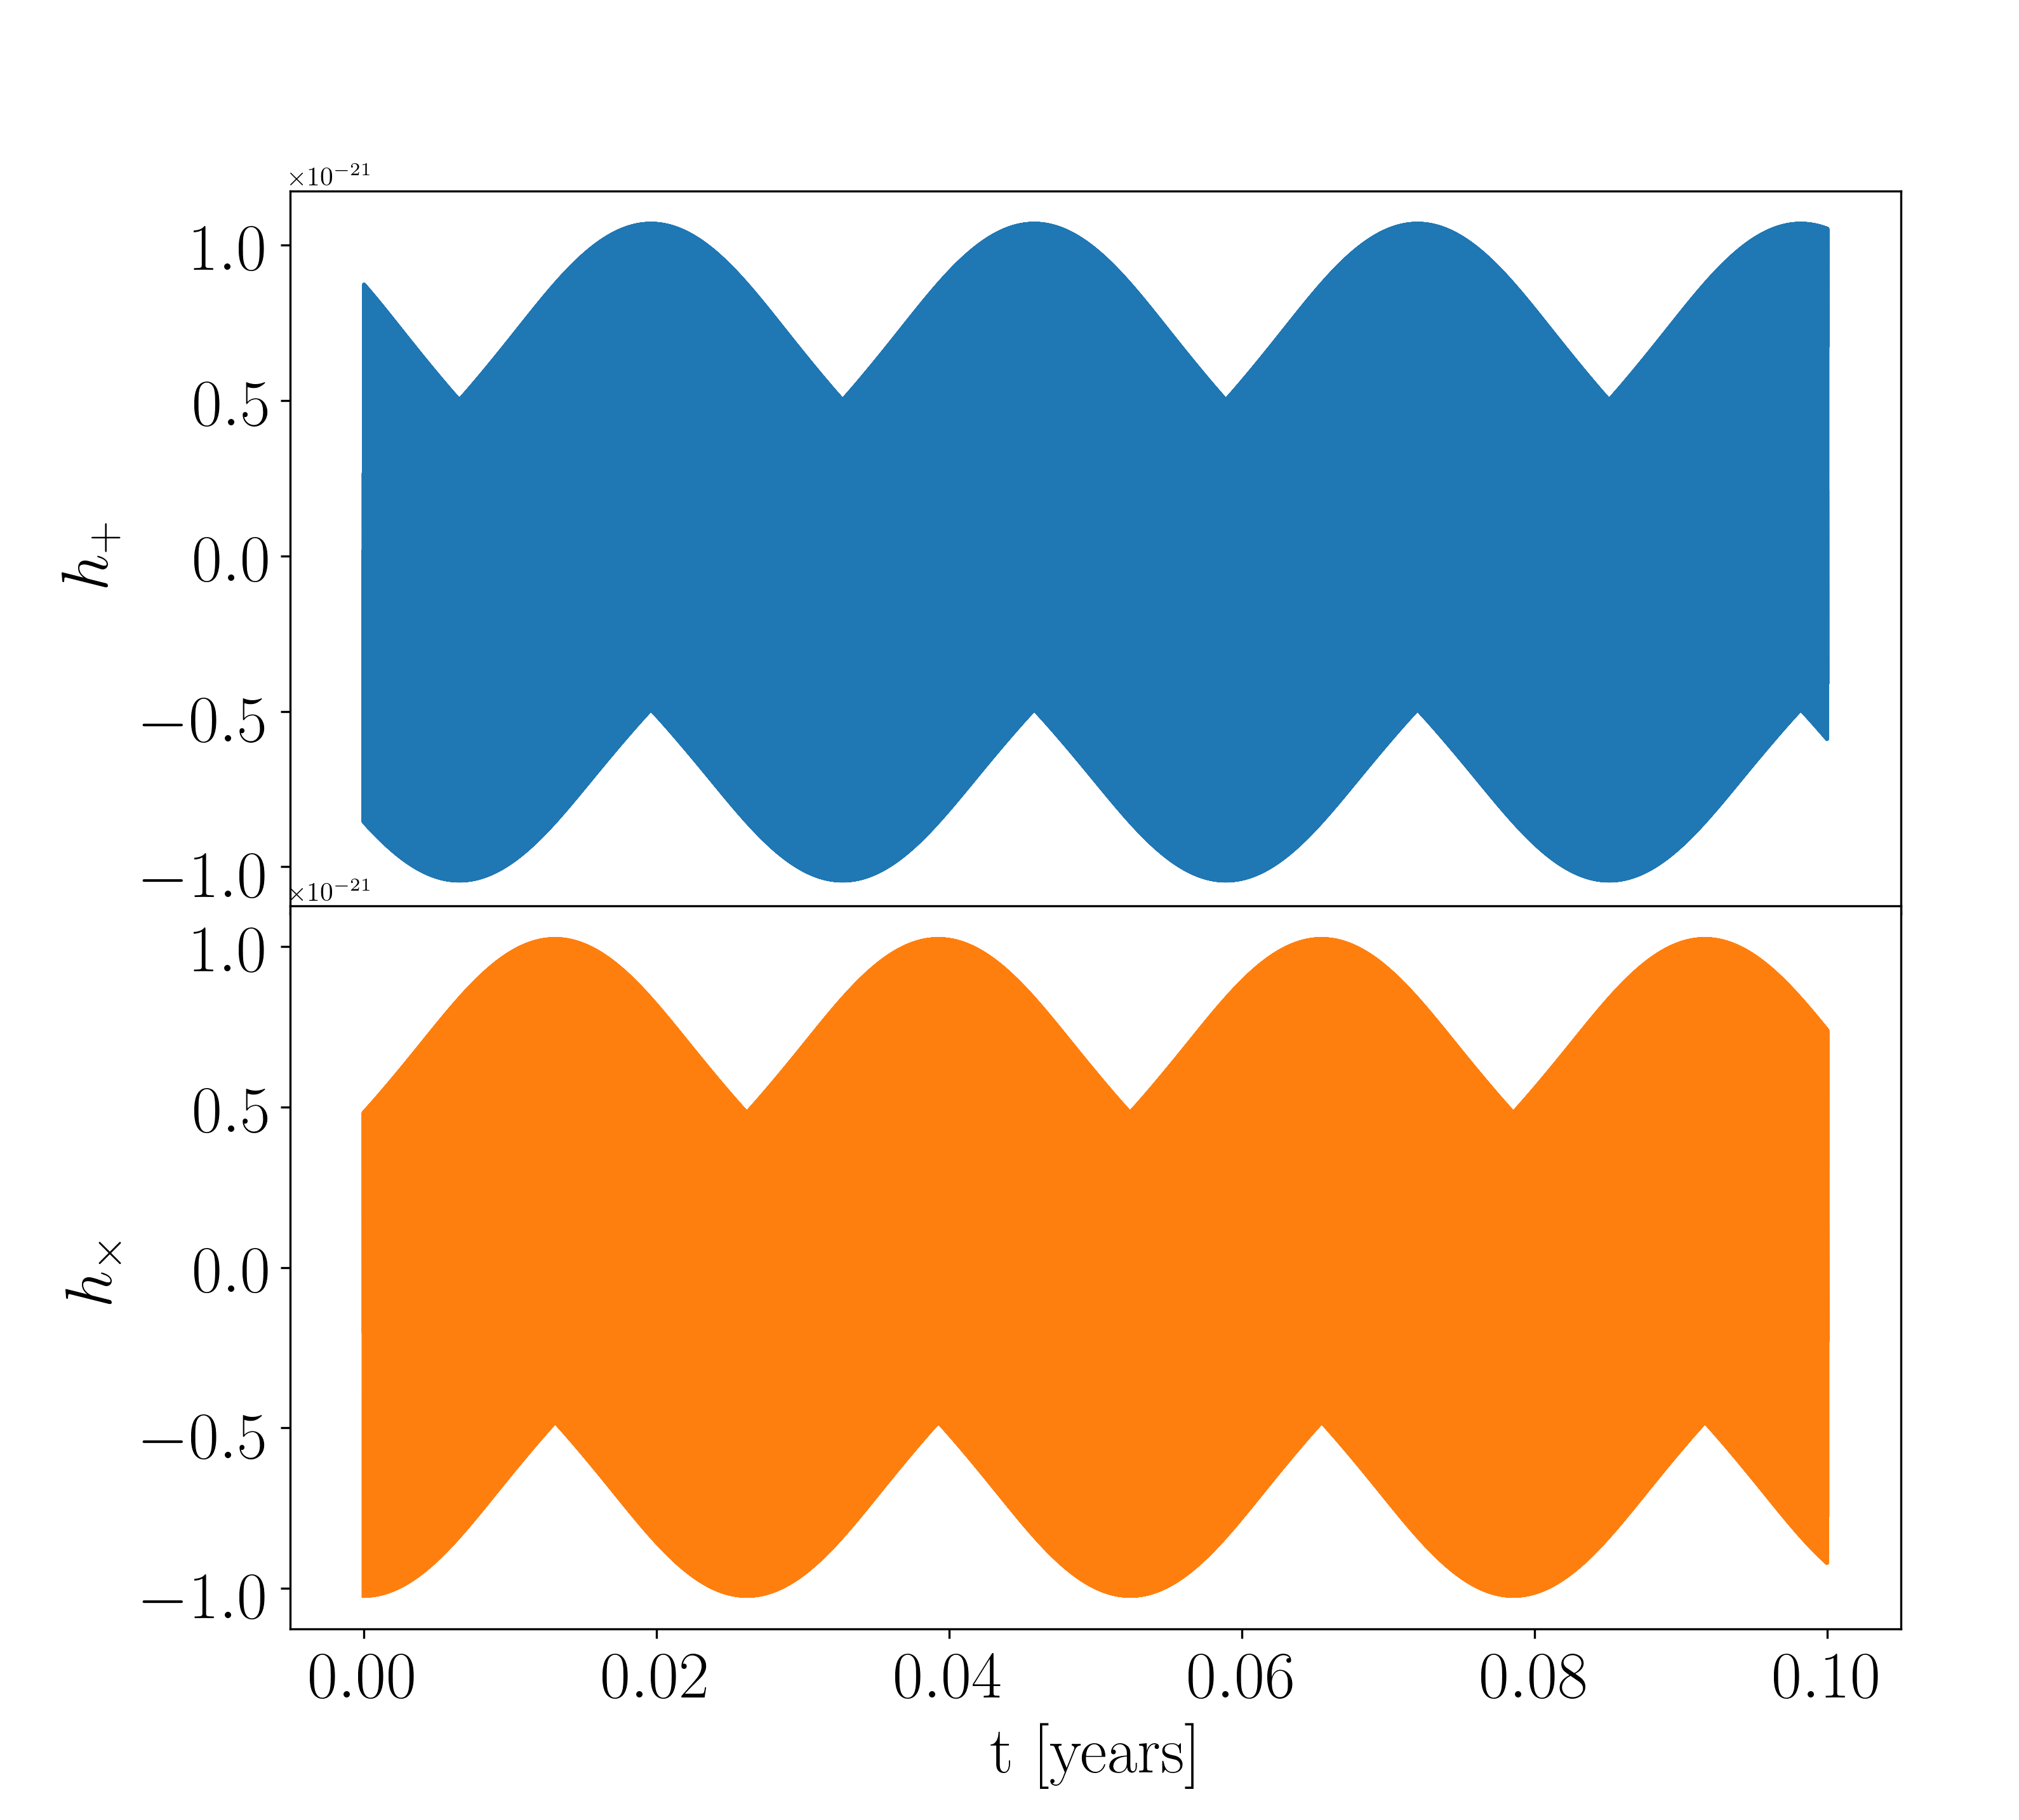
\includegraphics[width=0.8\textwidth]{GW_WaveformsLONG.png}} \\
%	\medskip
%	\caption{Gravitational waveforms over long and short timescales}
%	\label{fig:waveforms}
%\end{figure*}
%
%
%\begin{figure}
%	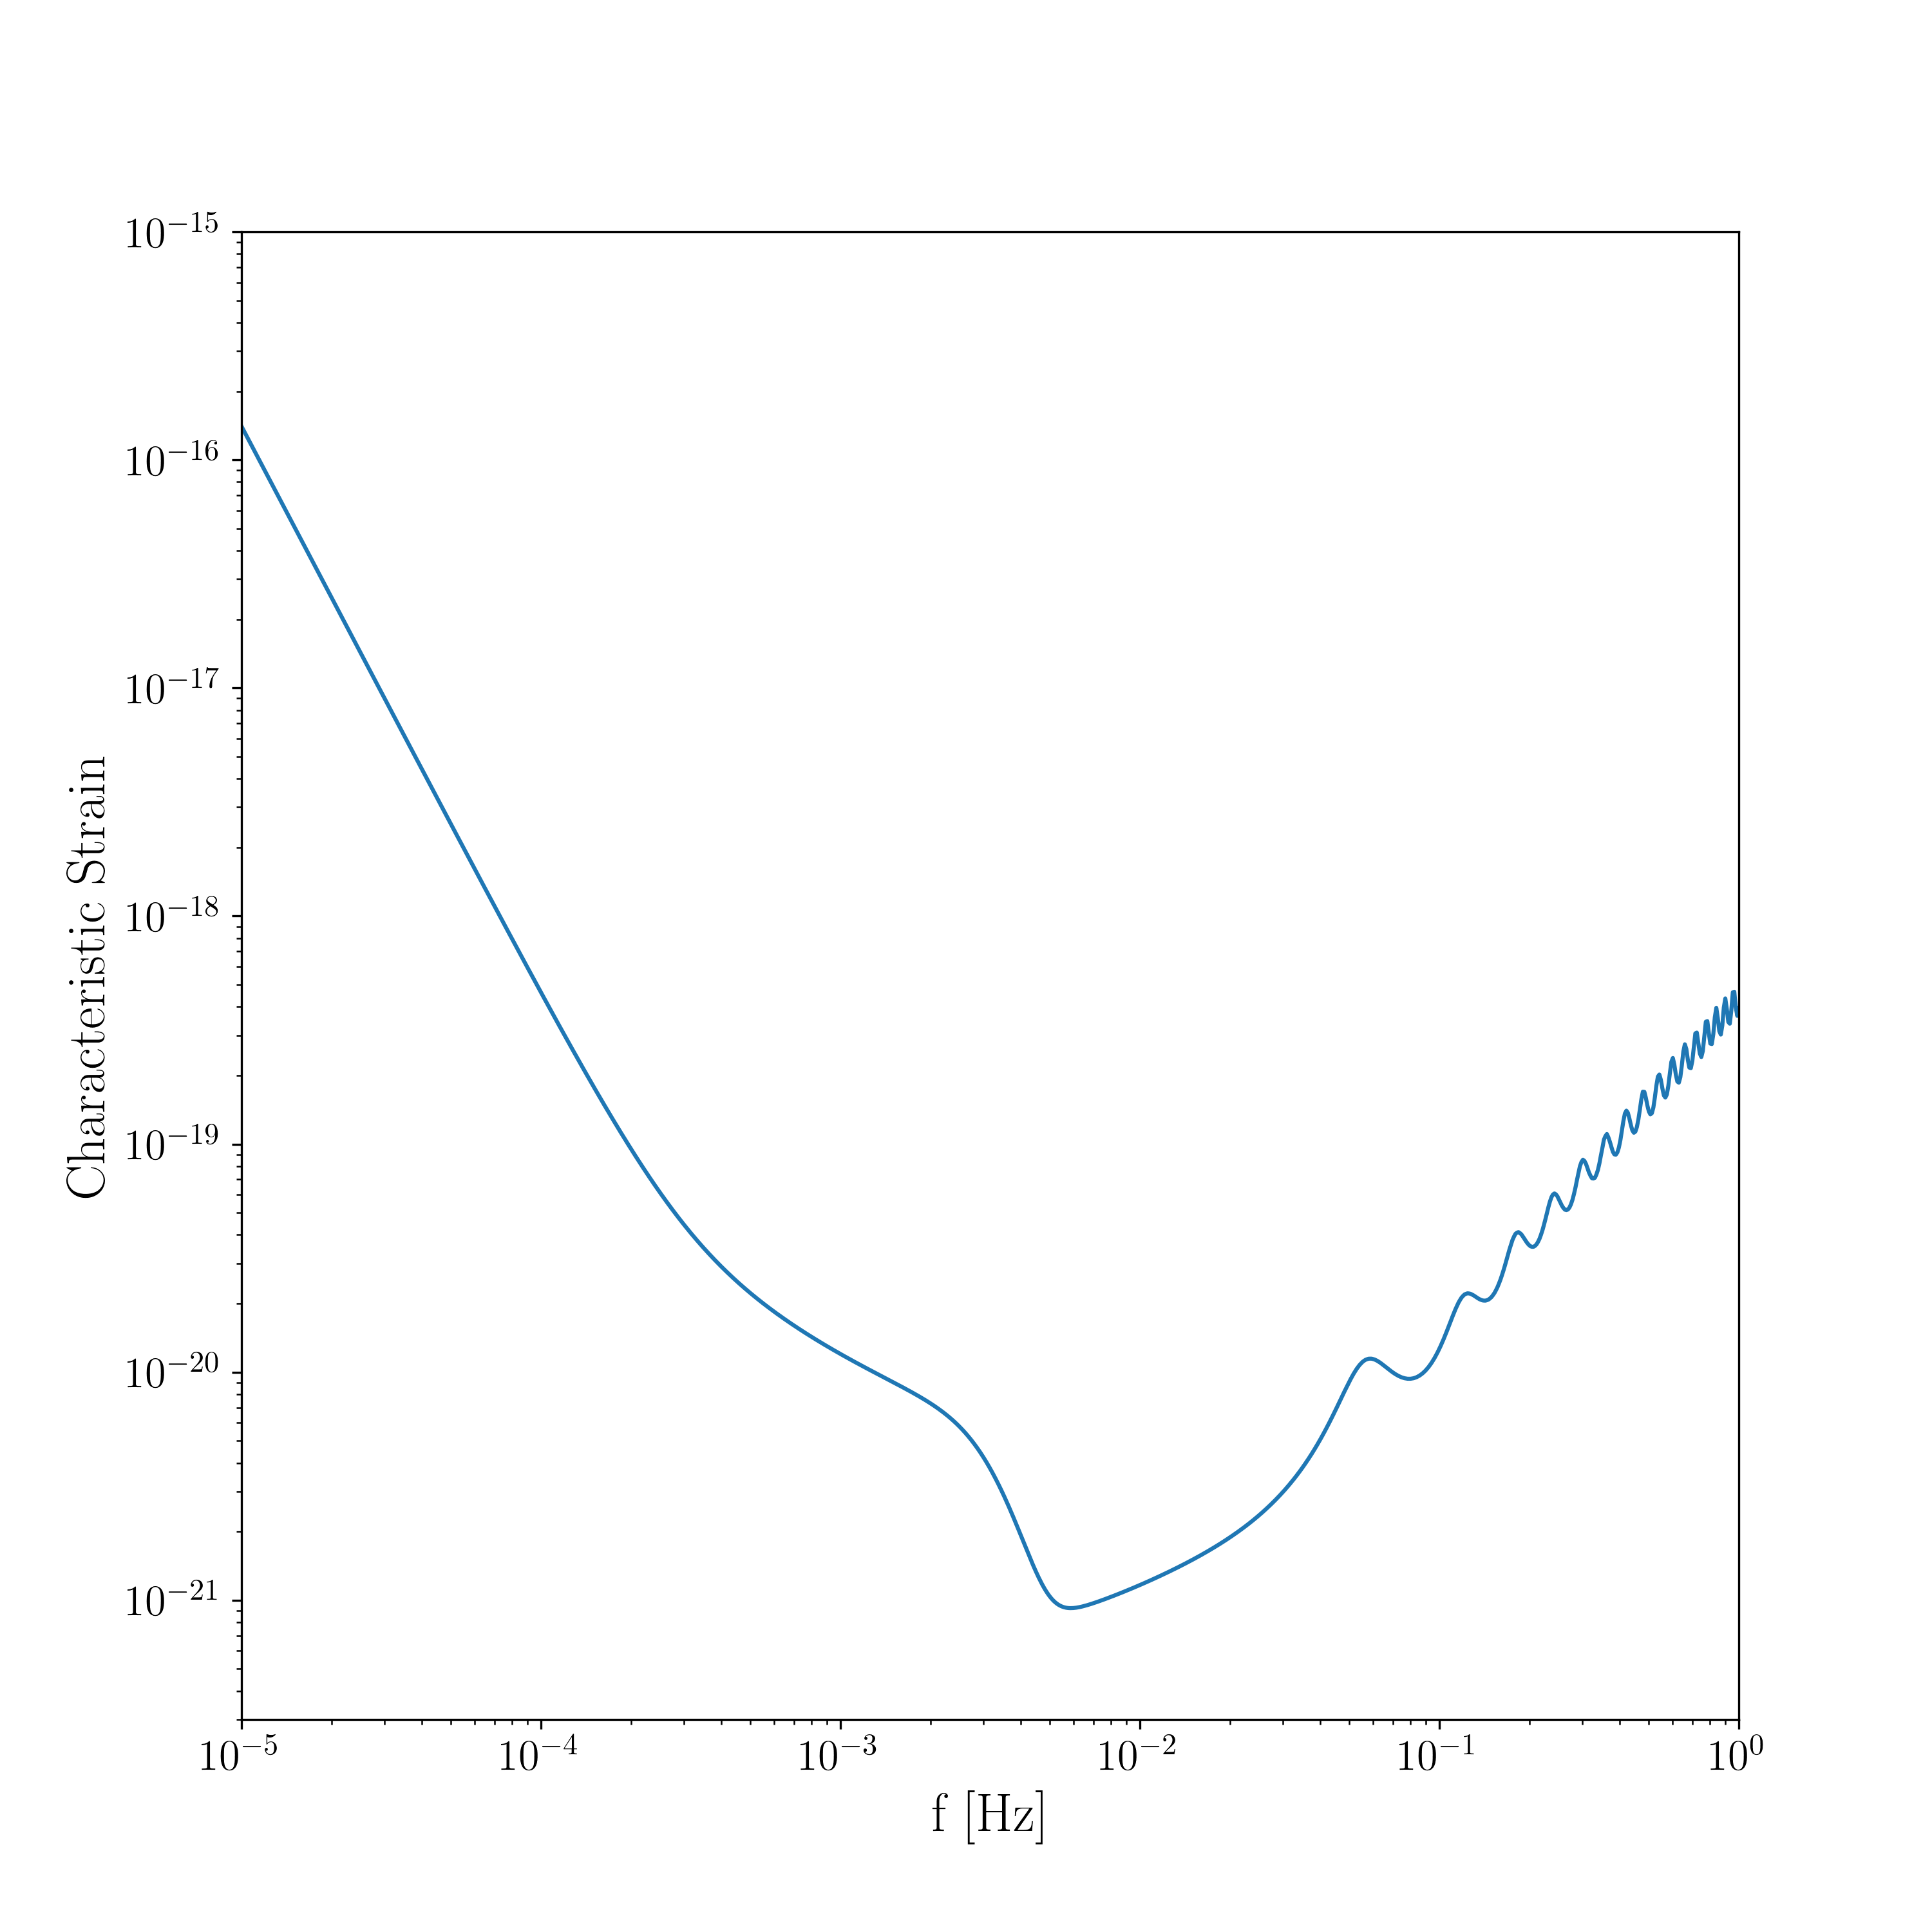
\includegraphics[width=0.8\textwidth]{LISANoise.png}
%	\caption{LISA noise curve}
%	\label{fig:noise}
%\end{figure}


\bibliographystyle{mnras}
\bibliography{paper2}


% Don't change these lines
\bsp	% typesetting comment
\label{lastpage}
\end{document}

% End of mnras_template.tex